\chapter{Literature review}
\label{sec:chapter1}
\section{Introduction}
Alzheimer’s disease (AD) is the most common neurodegenerative disease and a leading cause of dementia in the elderly \citep{andrieu2015}. This disease is characterized by a progressive loss of synapses and neurons in certain brain regions (e.g. cerebral cortex and hippocampus), leading to impaired memory and deterioration of cognitive functions \citep{dekosky1990,scheff2006,zare-shahabadi2015}, thus necessitating full-time medical care \citep{prince2013}. Currently, the disease is incurable. Although a lot of efforts have been directed towards developing AD disease-modifying therapies, current treatment strategies are aimed at ameliorating disease symptoms alone \citep{anand2014,disanto2013}. Age is the most prominent risk factor for AD and about 44 million people are currently affected globally. While only 5 \% of individuals over the age of 65 years are affected by AD, the prevalence doubles with every 5 years of increasing age \citep{pimenova2018,qiu2009}. Given the rapidly aging population in first-and third-world countries, the prevalence of AD is predicted to rise to 81 million by 2025 \citep{AlzheimersAssociation2014,Ferri2005}. Moreover, it has been estimated that by 2050, 22 \% of the global population will be over the age of 60, with the majority residing in the developing nations \citep{Annear2015,Paddick2013}. In South Africa, there are limited statistics on the prevalence of AD. According to the census conducted in 2011, there are approximately 2.2 million people with some form of dementia. Very little is known about the prevalence of dementia and how it impacts on older adults residing in low and middle classes, as well as in the rural areas, where most of the adult population reside. Despite this, it was reported that about 79 \% of patients were being cared for by family members \citep{Kalula2010}. In the continued absence of effective therapeutic strategies to either delay or slow down the disease progression, AD will pose a tremendous burden on healthcare and social services. 

AD is a multifactorial disease that is highly complex, with genetic as well as environmental causes \citep{Dorszewska2016}. This disease is classified into two subsets. The first being the early-onset Familial Alzheimer’s disease (FAD, onset $<$ 65), which contributes to the least cases of AD (1-5 \%) with strong genetic association \citep{Musiek2015,Reitz2014,Swerdlow2007}. The second being sporadic late-onset Alzheimer’s disease (LOAD, onset $\geq$ 65) which contributes to the majority of all AD cases ($>$ 95 \%), \citep{Musiek2015,Reitz2014,Swerdlow2007}, with an unclear cause \citep{Dorszewska2016,pimenova2018}. Certain genes such as amyloid precursor protein (APP), Presenilin 1 (PSEN1) and Presenilin 2  (PSEN2) are responsible for the occurrence of FAD, while APOE gene is responsible for LOAD \citep{Dorszewska2016}.

AD pathology occurs in 5 stages; the pre-symptomatic, Mild Cognitive Impairment (MCI), mild AD, moderate AD and severe AD \citep{Caldwell2015}. The first two stages encompass a prodromal stage, which, in the majority of cases, precedes symptom onset by several years (at least 20 - 30 years) \citep{Caldwell2015,Caselli2013,Penn1993}. During this time, pathological molecular changes occur inside the brain and are present as two molecular hallmarks which occur as a result of perturbations in cellular proteostasis. The senile plaques, which are extracellular deposits of amyloid beta ($A\beta$)
peptides, and intraneuronal neurofibrillary tangles (NFTs), which are somatic inclusions of hyperphosphorylated, microtubule-associated protein tau, respectively \citep{Mattson2008} (\Cref{fig:10_AD_hallmarks}). To better understand the multifactorial pathophysiology of AD, several hypotheses have been put forward, including the amyloid cascade hypothesis (ACH), the cholinergic and tau hypothesis, as well as inflammation \citep{Kurz2011}; however, many molecular aspects and their dynamic changes during disease progression remain unclear. The ACH, the most widely accepted mechanistic hypothesis for AD, posits that an imbalance between the production and clearance of ($A\beta$) peptides is a very early, often initiating factor in disease onset \citep{Hardy2009,Hardy1992}.

\begin{figure}[!htbp]
  \includegraphics[width=\linewidth]{figures/chapter10/10_AD_hallmarks}
  \caption[Pathological hallmarks of AD]{\textbf{Pathological hallmarks of AD.} Micrograph showing NFTs (arrows) and $A\beta$ plaques (arrowhead) in the AD brain \citep{Nixon2007}.}
  \label{fig:10_AD_hallmarks}
\end{figure}

Proteolytic systems; the ubiquitin-proteasome system (UPS) and the lysyosomal systems [the autophagy-lysosomal pathway (ALP) and the endocytic-lysosomal pathway (ELP)] are responsible for the degradation of mis-folded or aggregated proteins in order to maintain cellular homeostasis. For example, the UPS targets and degrades short-lived proteins in the cytoplasm and nucleus, while the lysosomal system removes primarily long-lived cytoplasmic proteins and damaged organelles \citep{Ravikumar2003,Rubinsztein2005}. A large body of evidence implicates these proteolytic systems in the AD pathophysiology. Dysfunction of these system has been well documented in AD pathophysiology and although extracellular $A\beta$ plaques and intraneuronal NFTs are defining hallmarks of AD neuropathology, a growing body of literature suggests that deficits in the autophagy–lysosomal pathway are likely to precede the formation of these pathological hallmarks \citep{Cataldo2000,Nixon2011,Perez2015,zare-shahabadi2015}, suggesting a potential causality. More recently, a systems biology study highlighted the pivotal role of dysregulated autophagy in neurodegenerative diseases, where toxic protein aggregates and damaged organelles accumulate within specific types of neurons and lead to neuronal dysfunction and ultimately, demise \citep{Caberlotto2014}.

Although we have advanced our understanding of the molecular machinery that regulates the rate of protein degradation through autophagy at basal levels and the many aspects of its dysfunction in AD, the deviation of autophagic activity from basal levels and its change during disease pathogenesis in neuronal tissue remains largely unclear. Over the recent years, we have made substantial progress in modulating autophagy using pharmacological agents \citep{Berger2006,Hebron2013,Ravikumar2002,Ravikumar2004,Rose2010} or lifestyle interventions \citep{Alirezaei2010,Kuma2004,Mizushima2004a,Scott2004} \textit{in vitro} and \textit{in vivo}; yet many questions regarding an effective implementation of autophagy control remain unanswered. Therefore understanding the deviation of autophagic activity from basal levels and its change during disease pathogenesis as well as targeting or modulating autophagy activity precisely with the aim to restore autophagic flux may drive the development of better targeted therapeutic interventions that will slow down the disease progression and ultimately curing the disease instead of treating the symptoms. In this review, we start by describing neuronal metabolism and their metabolic profile and move to the involvement of reactive oxygen species in neurodegeneration, focusing on the role of oxidative stress and mitochondrial dysfunction in the pathogenesis of AD. We then turn our focus to amyloid beta biogenesis and its pathology in AD.  We highlight the recent advances in the usage of super-resolution techniques in molecular biology. We introduce autophagy and its molecular machinery and discuss its efficiency and essential function in neuronal cells, followed by its role in neurodegenerative diseases. We discuss how autophagic flux may differ in brain regions, and how the deviation of flux may relate to the state of protein aggregation in pathology. Furthermore, we review studies that localize the defect in autophagy in AD and assess the relationship between autophagic flux and neuronal cell death. Finally, we indicate the importance of accurately measuring and targeting autophagy and provide an overview of how autophagy may be modulated for therapeutic purposes in various model systems aimed at restoring autophagic flux. 

\section{Neuronal metabolism}
A brain is made up of two cells types, neurons and astrocytes, which are highly interconnected and form functional networks through their spatial organization. The co-dependency of these cells types is reflected by their metabolic profiles where different yet complementary pathways are used \citep{Belanger2011,Schonfeld2013}. The brain has a high energy demand. This is evident by the fact that 20 \% of oxygen and 25 \% of the glucose utilized by the human body is dedicated to only cerebral function, yet the brain encompasses only 2 \% of the total body mass \citep{Belanger2011}. This means, uninterrupted supply of energy substrates from the circulation is required to meet the energy demands. Glucose is the main substrate of energy in the brain 
\citep{Dienel2012,Pellerin2012}, however, other energy substrates such as lactate, pyruvate, glutamate, and glutamine can be utilized \citep{Zielke2009}.

Glucose is delivered into a cell via specific glucose transporters (GLUTs) and once inside, it is phosphorylated by an enzyme called hexokinase (HK) to generate glucose-6-phosphate (glucose-6P) \citep{Belanger2011,Herrero-Mendez2009}. The latter can enter three main metabolic pathways; glycolysis, pentose phosphate pathway (PPP), and glycogenesis in order to produce adenosine triphosphate (ATP). In glycolysis, glucose-6P is metabolized to produce pyruvate, 2 ATP molecules and NADH (nicotinamide adenine dinucleotide) \citep{Belanger2011}. Pyruvate can be metabolised further in the tricarboxylic acid (TCA) cycle and oxidative phosphorylation (OxPhos) in the mitochondria using oxygen to generate 30 - 34 ATP molecules and CO\textsubscript{2} or it can be reduced to lactate by lactate dehydrogenase (LDH) in the cytosol \citep{Belanger2011}. In PPP, glucose-6P is metabolized to generate NADPH (nicotinamide adenine dinucleotide phosphate), while in glycogenesis, it is stored as glycogen, with the latter occurring in astrocytes \citep{Belanger2011} (\Cref{fig:10_glucose_metabolism}). More importantly, astrocytes and neurons have the ability to oxidize glucose and/or lactate \citep{Zielke2009}.

\begin{figure}[!htbp]
  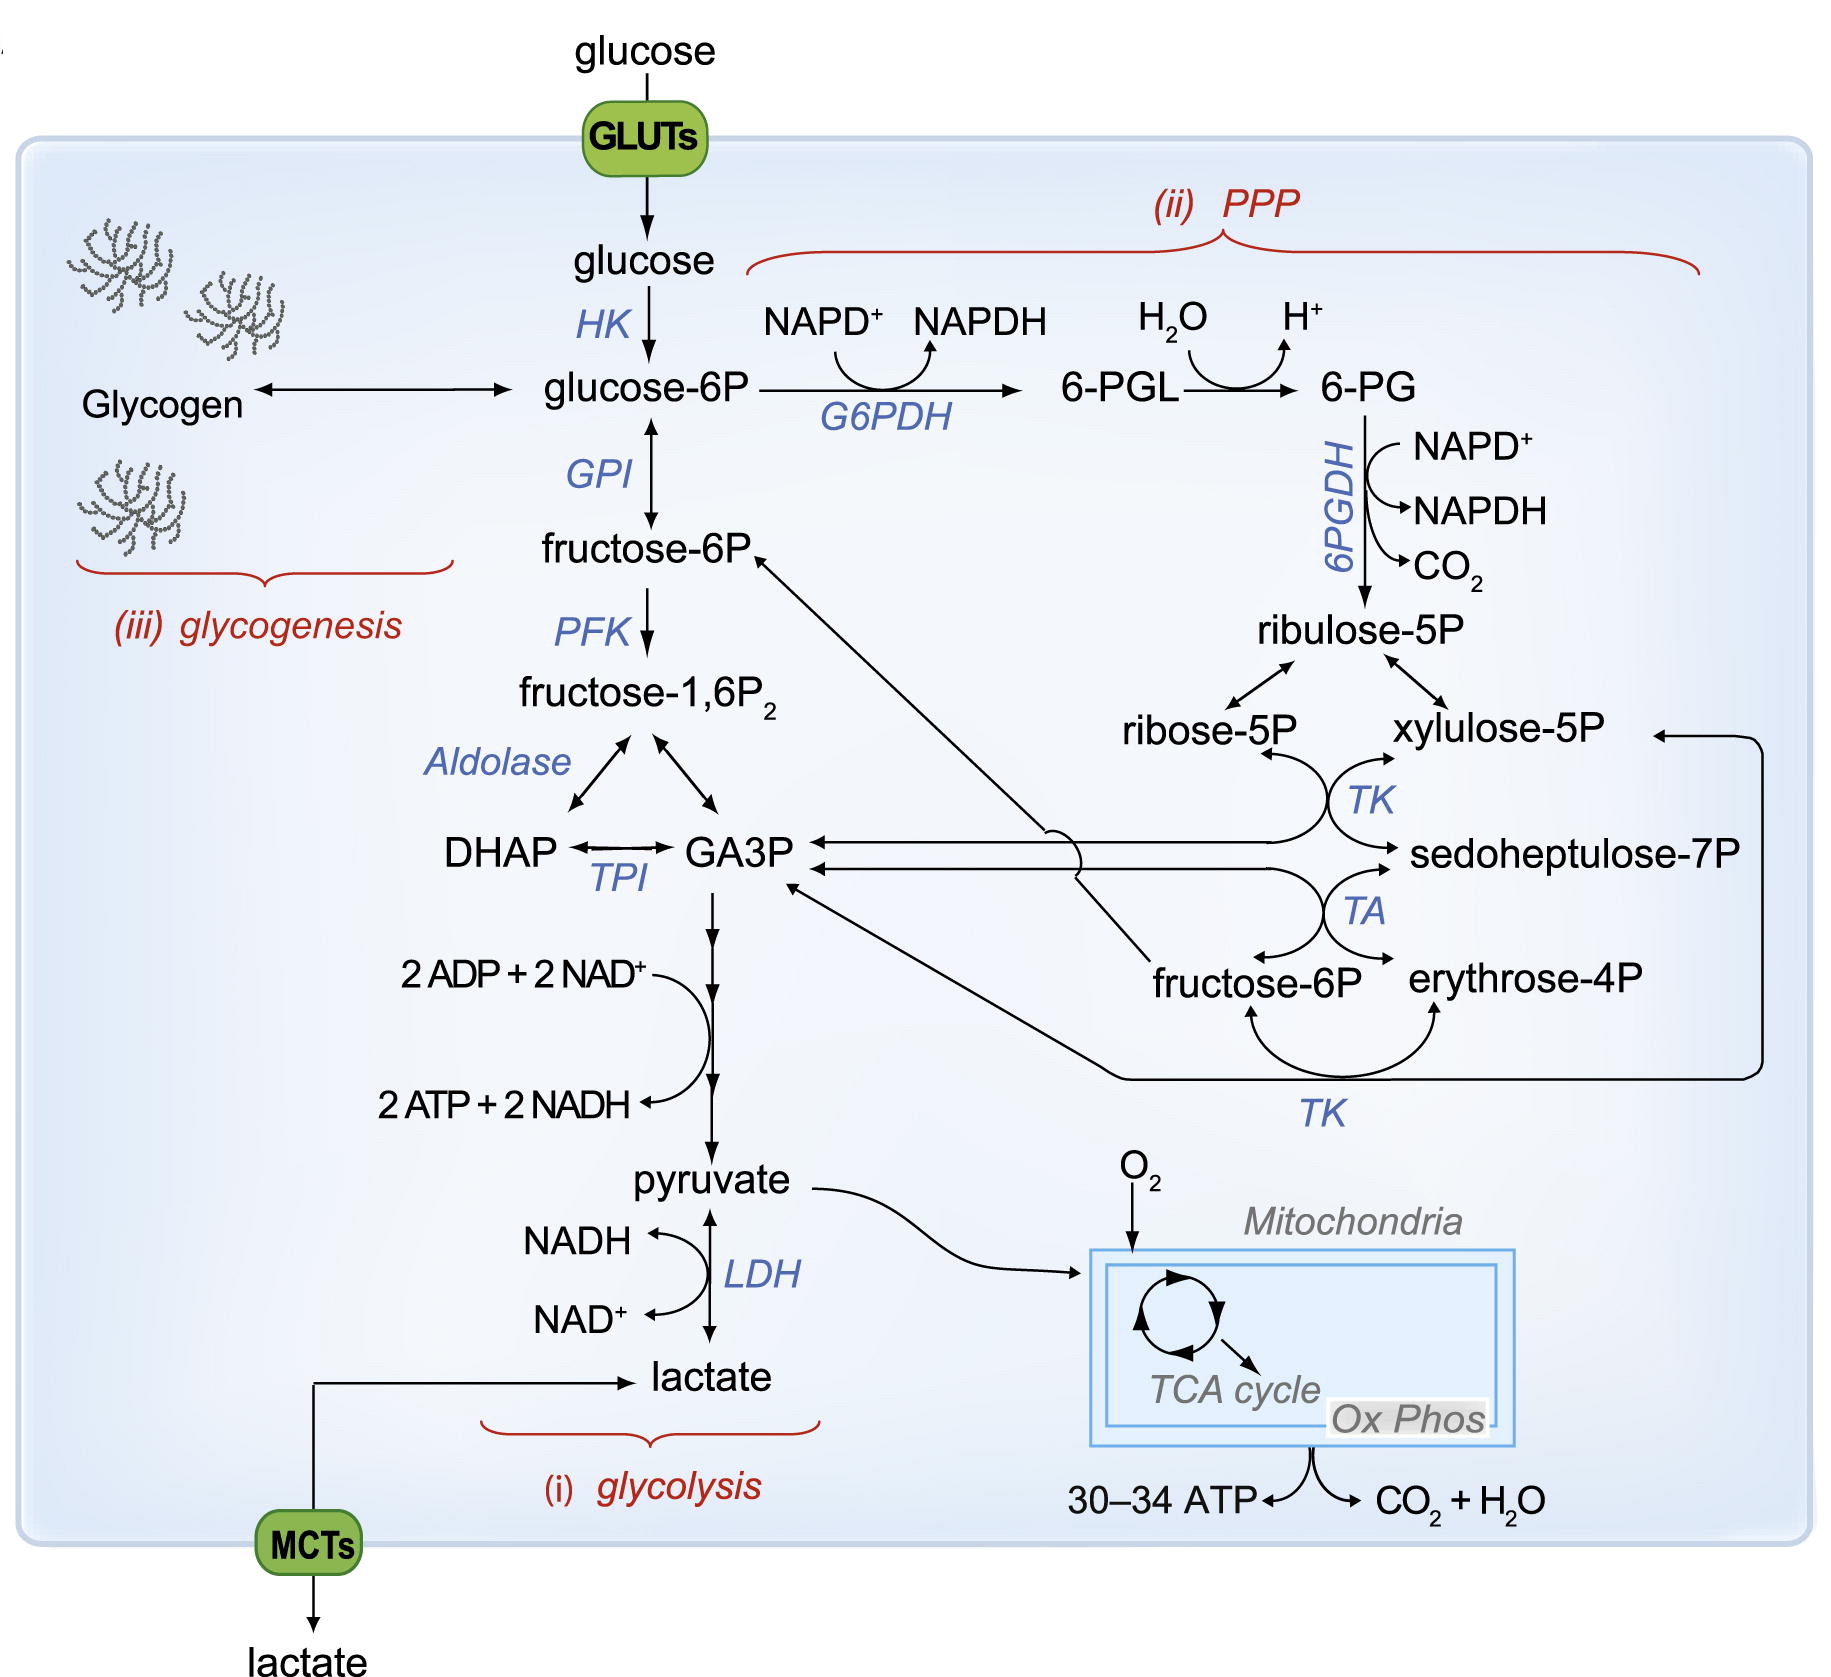
\includegraphics[width=\linewidth]{figures/chapter10/10_glucose_metabolism}
  \caption[Glucose metabolism]{\textbf{Glucose metabolism.} A schematic diagram showing three main pathways for glucose metabolism; glycolysis, pentose phosphate pathway, and glycogenesis \citep{Belanger2011} .}
  \label{fig:10_glucose_metabolism}
\end{figure}

\subsection{Metabolic profile of neurons}
Neurons are post-mitotic, highly differentiated cells that are characterized by high energy demands. This is due to their high levels of protein synthesis, which consumes a high amount of ATP within the mammalian cells \citep{Buttgereit1995}. Neurons depend almost exclusively on the energy produced through OxPhos (30 - 34 ATP molecules) compared to glycolysis (2 ATP) in order to meet their high energy demand needed to perform cellular functions, such as synaptic plasticity and neurotransmitter synthesis \citep{Cenini2019,Mattson2008,Schonfeld2013}. Mounting evidence demonstrate that neurons are capable of using lactate as an energy substrate \citep{Boumezbeur2010,Bouzier2000,Serres2005} and prefer lactate over glucose when both substrates are available \citep{Bouzier-Sore2006,Itoh2003}. Thus the specific characteristics of neurons are probably underly their distinct metabolic profile. For example, glycolytic enzyme 6-phosphofructose-2-kinase/fructose-2, 6-bisphosphatase-3 (PFKFB3) is highly expressed in astrocytes, but virtually absent in neurons because of a constant proteasomal degradation \citep{Almeida2004,Herrero-Mendez2009}. Because of this, neurons unlike astrocytes display a lower glycolytic rate, and thus cannot upregulate this pathway in response to cellular stress \citep{Almeida2004,Herrero-Mendez2009}. Indeed, a previous study showed that upregulation of glycolysis via PFKFB3 in neurons is in fact detrimental, resulting in oxidative stress and apoptosis \citep{Herrero-Mendez2009}. In this study, it was thought that the upregulation of glycolysis occurs at a cost of PPP metabolism that is needed to produce NADPH, an antioxidant vital for maintaining cellular redox state \citep{Herrero-Mendez2009}. Evidently, it has been shown that neurons have low NADPH compared to astrocytes \citep{Ben-Yoseph1996,Garcia-Nogales2003}, and since antioxidant system and the related enzymes are important for maintaining neuronal integrity and survival by keeping the levels of reactive oxygen species (ROS) relatively low \citep{Cenini2019}, it is not surprising that neurons are vulnerable to oxidative damage, implicated in neurodegeneration.

\section{ROS and its role in neurodegeneration}
ROS are a group of reactive molecules that are produced naturally in biological systems as part of normal cellular metabolism and are important in maintaining cellular homeostasis \citep{Cenini2019}. These include superoxide (O\textsubscript{2}\textsuperscript{-}), hydroxyl radical ($\cdot$OH), hydroxyl ion (OH\textsuperscript{-}) and hydrogen peroxide (H\textsubscript{2}O\textsubscript{2}), all of which are generated from oxygen. O\textsubscript{2}\textsuperscript{-} is generated from oxygen in the mitochondria as a result of the respiratory chain complex or NADPH oxidase and can be converted by superoxide dismutase (SOD) enzyme to produce H\textsubscript{2}0\textsubscript{2}. The latter can, in turn, be converted to other types of ROS, for example $\cdot$OH and OH\textsuperscript{-} \citep{Kim2015a}, with $\cdot$OH being the most reactive ROS responsible for cytotoxicity \citep{Bolisetty2013}.

Under physiological conditions, ROS levels are maintained at relatively low by antioxidant system \citep{Dasuri2013,Gandhi2012}, and are involved cellular processes such as inflammation, immune response, cell survival, synaptic plasticity, learning, and memory \citep{Cenini2019,Kishida2007,Liu2017}. However, increased ROS production can be harmful because of its ability to oxidise nucleic acids, protein and lipids \citep{Wang2014}. In fact, increased ROS accumulation has been implicated in oxidative stress, mitochondrial dysfunction and in gliosis. However, the role of ROS in gliosis is poorly understood and only one study provides evidence \citep{Kishida2007}.

Excessive accumulation of ROS due failure of antioxidant system or increased ROS production can result in oxidative stress, defined as an imbalance between rate of ROS production and clearance \citep{Wang2014}. High levels of oxidative stress have been implicated in aging and in the pathogenesis of various neurodegenerative diseases \citep{Bonda2010,Cenini2019,Liu2017,Shibata2008}. Neurons are most susceptible to oxidative stress and damage due to its high oxygen consumption, high energy demand, low antioxidant defenses as well as high abundance of polyunsaturated fatty acid which are susceptible to lipid peroxidation \citep{Cobley2018}. Thus, it is not surprising that ROS induced oxidative damage is widely reported in AD. In addition, since mitochondria are the major source of ROS production and the main target of oxidative stress, progressive mitochondrial dysfunction has also been implicated in the pathogenesis of AD \citep{Swerdlow2007}. The involvement of oxidative stress and mitochondrial damage in AD has been demonstrated in different models and are described below. 

\subsection{Evidence of oxidative stress in AD}
Oxidative damage is one of the earliest events in AD \citep{Nunomura2001}. This is supported by several studies that demonstrated elevated levels of oxidative stress in patients with mild cognitive impairment (MCI) \citep{Ansari2010,Pratico2004,Williams2006}. In addition, antioxidants including uric acid, vitamin C and E as well as antioxidant enzyme SOD were found to be decreased in MCI patients \citep{Rinaldi2003,Torres2011}. Increased oxidative stress has also been implicated in AD. Excessive production of ROS is thought to play an essential role in the accumulation and deposition of $A\beta$ peptides \citep{Bonda2010}. \citet{Ferreiro2008} reported that $A\beta$ plaques depleted Ca\textsuperscript{2+}  (calcium) ion storage in the endoplasmic reticulum (ER), leading to in cytosolic Ca\textsuperscript{2+} overload, which resulted in the reduction of endogenous GSH (glutathione) levels and ROS accumulation. In addition, increased H\textsubscript{2}O\textsubscript{2} levels and increased peroxidation of proteins and lipids were shown in transgenic mice expressing APP/PS-1, suggesting that $A\beta$ may exacerbate oxidative stress in AD \citep{Matsuoka2001,Zhao2013}. In addition, products of lipid peroxidation such as 4-hydroxynonal (4HNE), malondialdehyde (MDA), and 2 propenal (acrolein) have been found to be elevated in multiple studies performed in patients with AD \citep{Wang2014,Zhao2013}. For example, significantly increased levels of 4HNE were reported in the hippocampus \citep{Lovell1995,Markesbery1998,Montine1998}, parahippocampal gyrus \citep{Markesbery1998}, entorhinal and temporal cortex \citep{Montine1998}, amygdala \citep{Lovell1995,Markesbery1998}, ventricular fluid \citep{Lovell1997}, and plasma \citep{McGrath2001} in AD patients versus control subjects of the same age. Similar findings were observed with MDA and acrolein in AD patients. MDA was found to be increased in the hippocampus \citep{Lovell1995}, pyriform cortex \citep{Lovell1995}, temporal cortex \citep{Marcus1998,Palmer1994} and occipital cortices \citep{Miranda2000}, while elevated levels of acrolein were reported in the hippocampus/parahippocampal gyrus \citep{Bradley2010,Calingasan1999,Lovell2001,Williams2006}, amygdala \citep{Lovell2001}, superior and middle temporal gyri \citep{Bradley2010,Williams2006}, and cerebellum \citep{Bradley2010,Williams2006}. Altogether, these studies demonstrate the involvement of oxidative stress in AD.

\subsection{Evidence of mitochondrial dysfunction in AD}
As previously mentioned, mitochondria are the main source of oxidative damage due to the continuous generation of superoxide anion that results from electron leakage during electron transfer. Although mitochondria have an efficient antioxidant system, the production of superoxide anions is responsible for 90 \% of the endogenous ROS \citep{Wang2014}. It has been suggested that impaired mitochondria are more efficient producers of ROS, but less efficient producers of ATP. In fact, reduced energy metabolism in the brain is among one of the well-documented abnormalities in AD \citep{Wang2014}. A genome-wide transcriptomic study suggested that decreased cerebral glucose metabolism in AD was associated with reduced expression of neuronal genes encoding subunits of the mitochondrial electron transport chain (ETC). In support of this, several studies reported reduced expression of $\alpha$-ketoglutarate dehydrogenase complex, pyruvate dehydrogenase complex, and cytochrome oxidase in AD, which are the key enzymes of oxidative phosphorylation \citep{Chandrasekaran1994,Cottrell2001,Maurer2000}. Due to the role of mitochondria in calcium homeostasis, previous studies reported calcium mishandling i.e. increased calcium overload and decreased reuptake of calcium in fibroblasts of patients with AD \citep{Ito1994,Peterson1985}. \citet{Area-Gomez2012} reported a significant increase in function of mitochondria-associated ER membranes and ER–mitochondrial communication, measured by cholesteryl ester and phospholipid synthesis, respectively, in patients with familial and sporadic forms of AD \citep{Area-Gomez2012}. Consistent with this, ER–mitochondria interface proteins were found to be highly expressed in early stages of AD in patients as well as in the mouse model of APP\textsubscript{Swe/Lon}. Lastly, elevated oxidative damage to mitochondrial DNA was reported in patients with AD \citep{Mecocci1994,Wang2005}. Taken together, these studies provide evidence of the involvement of mitochondrial dysfunction in AD.

\subsection{Role of PQ in oxidative stress and in the pathogenesis of AD}
PQ is a pesticide that is widely used globally for agricultural practices. Several epidemiological studies have reported that pesticide exposure increases the risk of developing AD \citep{Baldi2003,Hayden2010,Santibanez2007,Yan2016}. In fact, genetic and environmental factors are the aetiology of the sporadic form of AD \citep{Landrigan2005}. Although the mechanism of PQ is better understood in PD than in AD, it is known that PQ accumulates in the cerebral cortex and hippocampus \citep{Landrigan2005}. Therefore, PQ could potentially impair learning and memory functions and affect AD pathogenesis. PQ exact its toxicity by inducing oxidative stress and mitochondrial damage \citep{Baltazar2014,Drechsel2008,Lin2006}, both of which are implicated in the pathogenesis of AD \citep{Lin2006}. Therefore, experimental models with PQ are widely used for understanding the roles of pesticide exposure in the development of AD as well as to study the mechanisms of AD. \citet{Drechsel2008} showed that PQ enhances H\textsubscript{2}O\textsubscript{2} production in brain mitochondria, and since H\textsubscript{2}O\textsubscript{2} is essential for regulating redox-sensitive signaling under normal condition \citep{Rhee2006}, it is not surprising that its increased generation has been implicated in the development of AD \citep{Du2008,Manczak2006}. Indeed, in wild-type mice and APP transgenic mice, exposure to PQ was found to increase oxidative stress as indicated by increased levels of 4HNE and nitrotyrosine in the mitochondria of the cerebral cortex \citep{Chen2012}. The authors also reported an increase in mitochondrial damage which was found to be directly correlated with impaired learning and memory as well as elevated $A\beta$ levels \citep{Chen2012}. Moreover, it was reported that over-expression of peroxiredoxin 3, a mitochondrial antioxidant defense enzyme, whose role is to remove H\textsubscript{2}O\textsubscript{2} protected against PQ induced mitochondrial damage, while decreasing $A\beta$ levels and improving cognition \citep{Chen2012}. These results provide evidence for the role of PQ induced oxidative stress in the pathogenesis of AD.

\section{$A\beta$ biogenesis}
Amyloid precursor protein (APP), an evolutionary conserved type 1 transmembrane protein, is unequivocally linked to AD pathogenesis as the unique source of neurotoxic forms of $A\beta$ \citep{Chen2015,Rajendran2012}. During early development, APP is highly enriched at the growth cones of developing neurites \citep{Ramaker2016,Sabo2003}. In more mature neurons, APP localizes to focal adhesion sites and within pre- and postsynaptic structures of the central and peripheral nervous tissue, suggesting a functional role in neuritic growth and synaptic plasticity \citep{Ashley2005,Yamazaki1997}. APP is synthesized in the ER and transported to the Golgi apparatus where it is packaged into vesicles for delivery to the cell surface for further processing by $\alpha$-, $\beta$-, and $\gamma$-secretases following the non-amyloidogenic (constitutive) or amyloidogenic pathway (\Cref{fig:10_amyloidogenic_pathway}) \citep{Obrien2011,Ramaker2016}. The cleavage activity of the $\beta$, and $\gamma$-secretases is mediated by the  $\beta$-site APP-cleaving enzyme 1 (BACE1) and presenilins (PSENs) catalytic domain, respectively \citep{Rajendran2012}. 

The non-amyloidogenic pathway leads to the production of non-pathogenic fragments, while the amyloidogenic pathway promotes the generation of $A\beta$ peptides. Briefly, following the former pathway, APP is first cleaved by $\alpha$-secretase, also known as distintegrin or metalloproteinase 10 (ADAM10), within the $A\beta$ sequence, thereby blocking $A\beta$ production, to generate two proteolytic fragments: soluble APP$\alpha$, and the corresponding C-terminal fragments, $\alpha$-CTF/C83 (a protein stub that remains secured to the plasma membrane for further proteolytic processing) \citep{Gandy1994,Roychaudhuri2009}. Soluble APP$\alpha$ is recycled back to the cell surface by the recycling compartments or delivered to the lysosome for degradation through the endosomal– lysosomal system \citep{Caster2013,Golde1992}. In the amyloidogenic pathway, APP is cleaved by $\beta$-secretase, the major secretase in the brain, at the N-terminus of the $A\beta$ sequence, thus generating soluble APP$\beta$, which is released extracellularly, and the corresponding C-terminal fragment, $\beta$-CTF/C99 (a membrane-associated fragment comprising the entire $A\beta$ sequence). Both C99 and C83 are subsequently cleaved by $\gamma$-secretase within the transmembrane domain, resulting in the release of a nontoxic p3 fragment, APP intracellular domain, and $A\beta$ peptide species of slightly different lengths (\Cref{fig:10_amyloidogenic_pathway}) \citep{Cole2007,Jarrett1993}. Secretase cleavage gives rise to an admixture of $A\beta$ peptides composed of 39–43 amino acids, with $A\beta$40 (90 \%) and $A\beta$42 (10 \%) being the two major $A\beta$ species \citep{Gouras2000,Takahasi2013}. Neuronal cells produce both $A\beta$40 and $A\beta$42 peptides, with healthy neurons having a high $A\beta$40/$A\beta$42.

\subsection{Role of $A\beta$ pathology in AD}
Although $A\beta$42 is produced at low quantities in neurons, it has a higher tendency to self-aggregate and forms higher-order structures, including toxic $A\beta$ dimers, trimers, and oligomers. These higher-order structures able to coalesce to form fibrils in insoluble beta-sheet conformation that eventually deposit into diffuse senile plaques \citep{Burdick1992,Gravina1995}. However, various studies have shown that the oligomers are the main source of its neurotoxicity \citep{Shankar2008,Shankar2009}. Although autophagy is responsible for the bulk degradation of aberrant proteins, not all aggregate-prone proteins are fully amenable to autophagic degradation \citep{Wong2008}. For example, expression of human $A\beta$40 and $A\beta$42 in Drosophila brain has been shown to have differential effects on neuronal autophagic degradation \citep{Ling2009}. Studies have shown that although autophagy sequesters $A\beta$42, this aggregate-prone peptide, in turn, may decrease the degradative capacity of autophagy \citep{Ling2014,Ling2011}. This was demonstrated by highly concentrated intracellular $A\beta$ identified in autophagic vacuoles (AVs), which accumulate in affected neurons, especially with advancing age \citep{Ling2011}. In contrast, sequestration of $A\beta$40 does not produce any detectable changes in either the neuronal autophagy activity or neurological defects \textit{in vivo}, which is consistent with the ACH for AD pathogenesis \citep{Hardy1992}.

Prior to senile plaque deposition, $A\beta$42 oligomers are able to induce oxidative damage, promote tau hyperphosphorylation, and lead to synaptic and mitochondria toxicity \citep{Kaminsky2015,Lustbader2004}. Moreover, during late disease progression, $A\beta$42 senile plaques have been found to activate microglia \citep{Rosenmann2013}. Microglial activation results in the production and release of proinflammatory cytokines, including IL-1$\beta$, TNF-$\alpha$, and IFN $\gamma$, which in turn stimulate the nearby astrocytes to further exacerbate $A\beta$42 production and dispersal \citep{DalPra2015}. To this end, immunohistochemical analysis has revealed significantly higher $A\beta$42 levels in AD brains than control brains \citep{Funato1998}. Additionally, the extent of $A\beta$42 deposition is much greater in AD brains with disease progression, while $A\beta$40 shows little or no apparent age-dependent accumulation \citep{Funato1998}.

It is well established that AD-causing mutations in APP and in presenilin 1 (PSEN1) and presenilin 2 (PSEN2) alter APP proteolytic processing in a manner that alleviates the relative levels of the $A\beta$42 peptides \citep{Borchelt1996,Scheuner1996}. Mutations in APP that lie within the $A\beta$ sequence increase the self-aggregation of the resultant peptides, not their production, while mutations in PSEN1 and PSEN2 increase the relative production of the longer, more hydrophobic, and self-aggregating $A\beta$42 peptides \citep{Kim2008,Weggen2012}. Furthermore, the inactivation of PSEN1 and PSEN2 has been shown to completely prevent $A\beta$ generation \citep{Herreman2000,Zhang2000}. Although $A\beta$42 is generated at a 10-times lower rate than $A\beta$40, the former peptide has consistently been shown to be the main component of $A\beta$ plaques in AD \citep{Iwatsubo1994}. Originally, the ACH was mostly driven by genetic studies indicating the vast majority of early-onset familial AD mutations to confer a similar biochemical phenotype, i.e., an increased ratio of cerebral $A\beta$42, either through an increased $A\beta$42 production or decreased $A\beta$40 production, or a combination of both \citep{Cavallucci2012,Cruts1998}. And although the ACH takes a central position in AD-related research, the prevailing hypothesis does not entirely account for the complex pathophysiology of AD. Instead, it seems that the role of $A\beta$ in synaptic degeneration may act in concert with several other factors that impair the integrity of neuronal functions \citep{anand2014,DalPra2015}. Growing evidence supports that dysregulated production of both $A\beta$ and tau may synergistically disrupt synaptic activity and mitochondrial function, resulting in AD \citep{Chetelat2013,Musiek2015,Quintanilla2012,Teplow2013}. Although many factors contribute to AD pathogenesis, imbalance in $A\beta$ production and clearance has emerged as the most extensively validated and compelling therapeutic target for both genetic and sporadic AD, as both forms of the disease can be ascribed similar etiologies \citep{Selkoe2012,Selkoe2016}.

\begin{figure}[!htbp]
  \center
  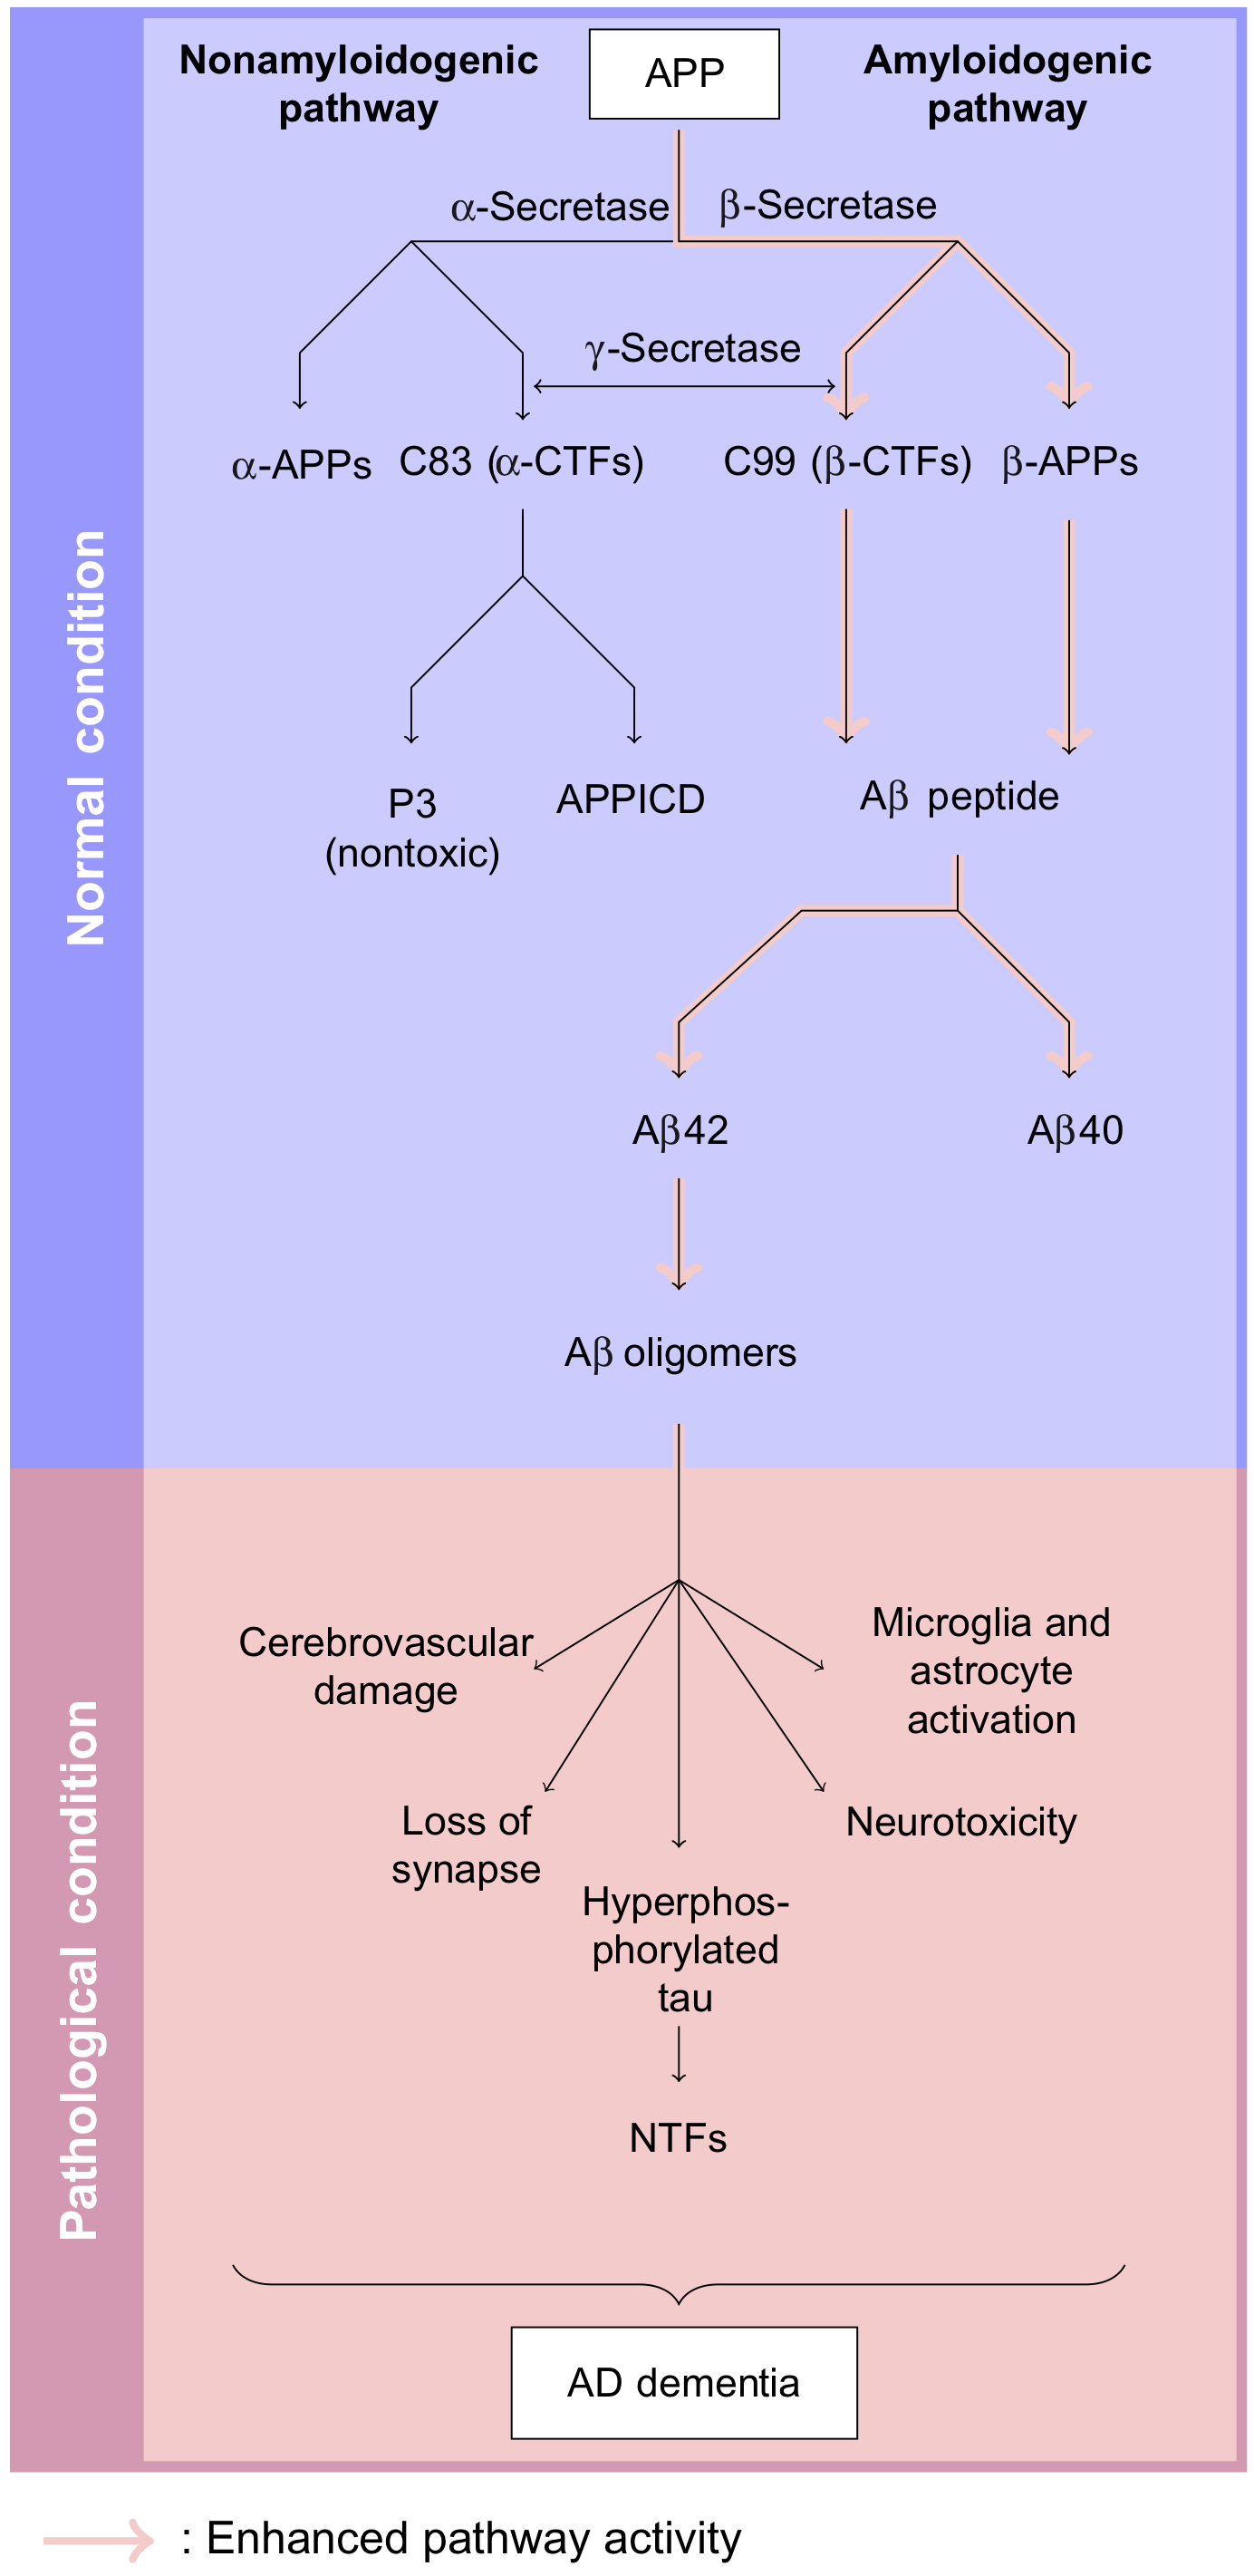
\includegraphics[width=0.7\linewidth]{figures/chapter10/10_amyloidogenic_pathway}
  \caption[The nonamyloidogenic and amyloidogenic pathways.]{\textbf{The nonamyloidogenic and amyloidogenic pathways.} Enhanced amyloidogenic pathway activity increases neuronal synthesis of aggregate prone toxic $A\beta$ oligomers, which in turn lead to autophagy and mitochondrial dysfunction as well as tubulin disruption, thereby driving neurofibrillary tangle (NFT) formation}
  \label{fig:10_amyloidogenic_pathway}
\end{figure}

\section{Advanced microscopy in the study of molecular biology}
\subsection{Role of super-resolution microscopy }
Microscopes play a key role in molecular biology. Fluorescence microscopy, in particular, remains one of the most important tools for biologists for various reasons. Firstly, it is essential for studying communications of biological molecules inside living cells, tissues, and whole organisms and subcellular structures at high resolution \citep{Han2013}. Secondly, it can acquire data rapidly and molecules of interest are targeted and labelled with specific fluorescence probes in a noninvasive manner \citep{Han2013}. Thirdly, live cell imaging is possible. In conventional microscopes, the spatial resolution is limited in diffraction, about 200 nm in the $xy$ and 500 nm in the $z$ direction, making it impossible to identify smaller sub-cellular structures or monitor biological processes which occur at nanometer scale \citep{Xu2017}. Therefore, in the past two decades, efforts to break the diffraction limit in order to understand cell structure and dynamics at a molecular level, in 2 and 3 dimensions. Currently, super-resolution microscopes capable of imaging cellular structures and rapid cellular dynamics at single molecule level at 10 nm are available. These include stimulated emission depletion (STED) microscopy \citep{Klar1999}, saturated structured illumination microscopy (SSIM) \citep{Gustafsson2005}, and single molecule localization microscopy such as  photoactivation localization microscopy (PALM) \citep{Betzig2006} and stochastic optical reconstruction microscopy (STORM) \citep{Huang2008,Xu2017}. STED and SSIM use patterned illumination to improve the resolution by controlling few molecules which are excited and detected simultaneously, while PALM and STORM activate single molecules at different times \citep{Han2013}, \Cref{fig:10_superresolution}. The application of these techniques in molecular biology has been extensively reviewed elsewhere \citep{Han2013}. For the purpose of this review, we focus on single molecule localization techniques.  

Briefly, STORM/PALM is based on the photo switching and detecting single spatially separated fluorophores. This is achieved by photoswitching  fluorophores between their  "ON" and "OFF" state, where most of the fluorophores are forced to remain in the dark state for a longer time and allowing only a small subset of fluorophores  in  the “on” state to emit fluorescence at a given time \citep{Turkowyd2016}. In this manner, thousands of frames are imaged overtime  and reconstructed using image-processing algorithms allowing the precision localization of molecules, which depended on the sufficient collection of photons from each activation event and therefore, the reliability of the fluorophores employed \citep{Turkowyd2016,Xu2017}.

Currently, the use of correlative techniques such as correlative light and electron microscopy (CLEM) is gaining popularity in molecular biology. CLEM is a unique and powerful technique that combines two different imaging modalities, fluorescent light microscopy (LM) and electron microscopy (EM) in order to overcome the limitations of each, however at an expense of imaging fixed sample \citep{Russell2017}. Light microscopy allows one to identify fluorescently labelled molecules for their biological function within living cells and tissues which would not have been possible with EM, however, the information is limited in resolution, 200 nm with confocal microscopy and 10 nm with advanced super-resolution microscopy.  EM, particularly the transmission electron microscopy (TEM) allows ultrastructural visualization at a much fine resolution, 0.1 - 10 nm \citep{Feng2018}, thus combining these techniques has makes it possible for imaging rare dynamic biological events at high resolution. Traditionally, CLEM was performed on manually sectioned serial sections and imaging each section (more than 100 sections) using TEM or SEM (scanning electron microscopy). Nowadays, automated systems  based on the SEM such as focused ion beam SEM (FIB-SEM) \citep{Heymann2006} and serial blockface SEM (SBF-SEM) \citep{Denk2004} have gained popularity and are being used in molecular biology. In FIB-SEM and SBF-SEM, a gallium ion beam  or a diamond knife is used to sputter or remove slices of material from the blockface and the revealed surface is imaged repeated sequentially using a backscattered electron (BSE) detector to build up a stack of images through the volume of the sample \citep{Russell2017}.

\begin{figure}[!htbp]
  \includegraphics[width=\linewidth]{figures/chapter10/10_superresolution}
  \caption[Super-resolution fluorescence microscopy.]{\textbf{Super-resolution fluorescence microscopy.} Diagram showing the principles of super-resolution microscopy techniques (upper panel) and images  of microtubules imaged with each microscopy (lower panel) \citep{Feng2018}.}
  \label{fig:10_superresolution}
\end{figure}

\section{Autophagy}
\subsection{Definition and role}
Autophagy is a major catabolic process responsible for the degradation cytoplasmic material, including organelles within the lysosomal compartment \citep{He2009,Nixon2011}. Three types of autophagy exist, depending on the route through which the encircled cargo is delivered to the lysosomal compartment for degradation: microautophagy, chaperone-mediated autophagy (CMA), and macroautophagy \citep{Boya2013} as shown in \Cref{fig:10_autophagy}. In microautophagy, cytosolic components are directly transferred into the lysosomes through invagination of the lysosomal membrane \citep{Cai2012,Nixon2011}. In CMA, the protein targeted for degradation is recognized by a chaperone complex protein, HSC70, through a KFERQ motif located on the target protein peptide sequence. Subsequently, the substrate-chaperone complex is transported to the lysosome where it binds to the lysosome associated membrane protein type 2A (LAMP2A) receptor allowing the translocation of the protein across the lysosomal membrane into the lumen, where they are degraded \citep{Cuervo2014,Dice2007,Klionsky2010}. And lastly, macroautophagy (hereafter referred to as autophagy) which is the major degradation pathway of long-lived proteins and organelles, which operates entirely different compared to microautophagy and CMA, through distinct and dynamic membrane rearrangements. Here, a flat membraned cistern known as the phagophore sequesters substrates. The membrane source of phagophores is believed to arise from the  endoplasmic reticulum (ER), plasma membrane, mitochondria and ER-mitochondria contact sites \citep{Hailey2010,Hamasaki2013,Hayashi-Nishino2009,Ravikumar2010,sarkar2013,Yla-Anttila2009}.

The phagophore elongates and encircles the cytoplasmic material, forming a double-membraned vesicle, called an autophagosome \citep{Cai2012,Levine2008}, which subsequently fuses with lysosomes or with late endosomes to form a single-membrane hybrid organelles, amphisome, that latter fuses with lysosomes to form acidic autolysosome \citep{Cai2012,Nixon2011,sarkar2013}, where degradation of the encircled cargo takes place. The resulting macromolecules are recycled back into the cytosol to be reused as substrates for ATP generation or protein synthesis. The rate of protein degradation through autophagy is termed autophagic flux \citep{klionsky2016,loos2014}. Importantly, most cells and tissues have a distinct basal level of autophagic flux \citep{Mizushima2004a}, which has recently been elegantly visualized in various tissues \citep{Kaizuka2016}.  Autophagy, therefore, plays a critical role in maintaining cellular homeostasis by removing misfolded or damaged proteins and turnover of organelles \citep{Levine2008}. It also plays a role in maintaining energy homeostasis during starvation conditions by recycling cytosolic components to compensate for nutrient scarcity \citep{Levine2008,Loos2009}. Although autophagy plays a major role in cellular survival, it has been implicated in various human physiological and pathological conditions, such as development, aging, infection and immunity, longevity, aging, cancer, liver, neurodegeneration and heart disease \citep{Meijer2006,Mizushima2008,Ravikumar2010b,sarkar2013}.

\begin{figure}[!htbp]
  \includegraphics[width=\linewidth]{figures/chapter10/10_autophagy}
  \caption[Schematic representation of the three types of autophagy]{\textbf{Schematic representation of the three types of autophagy.} In microautophagy cytosolic components to be degraded are transferred directly into the lysosome through invagination of the lysosomal membrane, while in CMA, cytoplasmic proteins containing a KFERQ peptide motif are translocated into the lysosomal lumen for degradation. In macroautophagy, cytoplasmic material is sequestrated by an isolation membrane forming an autophagosome, which later fuses with the lysosome to form an autolysosome where degraded takes place \citep{Nikoletopoulou2015}.}
  \label{fig:10_autophagy}
  \end{figure}

\subsection{The autophagic machinery and its regulation}
Autophagy is an evolutionary conserved process from yeast to mammals with up to 36 ATG (autophagy-related genes) \citep{Thumm1994,Tsukada1993,Klionsky2007,Mizushima2010}. Subsets among these ATG proteins referred to as the ‘core’ molecular machinery are essential for autophagosome formation. These are classified into the following groups; (1) the ULK1 kinase complex, (2) ATG9 cycling complex, (3) the class III phosphatidylinositol 3-kinase (P3K)/ Vps 34 complex I, (4) the phosphatidylinositol 3-phosphate (PI3P) binding ATG2-ATG18 complex and (5) ATG12-ATG5 and ATG8/LC3 (microtubule-associated protein 1 light chain 3) \citep{Feng2014,Yang2010}. The autophagic pathway can be categorized into the following essential steps: initiation, expansion of the autophagosome membrane, maturation of the autophagosomes, and degradation. Each step requires tight regulation of several, indispensable, ATG genes \citep{Feng2014,Maday2014,Parzych2014}. 

Although autophagy is constitutively kept at low levels, diverse environmental stressors (e.g. reactive oxidative species, damaged organelles and protein aggregation) can act as inducers of this degradative machinery \citep{Mizushima2008}. Starvation is the classic stimulus for autophagy induction \citep{Kuma2004,Mizushima2004a}, allowing cells to respond to nutrient scarcity through increased allocation of amino acids from proteins sequestered as autophagic cargo \citep{Hosokawa2009}. The classical pathway regulating mammalian autophagy involves the serine/threonine kinase, mammalian target of rapamycin (mTOR): mTORC1 and mTORC2, in which mTORC1 negatively regulates autophagy \citep{Guertin2009,Noda1998,Ravikumar2010b}. During conditions of nutrient availability, active mTORC1 phosphorylates Unc-51-like kinase (ULK1), which is sequestered into a complex with the autophagic protein, ATG13, and focal adhesion kinase family interacting protein of 200kDa (FIP200), thereby inhibiting autophagy. In the absence of nutrients, amino acid deprivation, growth factor withdrawal, or treatment with rapamycin, ULK1 phosphorylation by mTORC1 is reduced and the ULK1 complex is activated through auto-phosphorylation, which in turns phosphorylates ATG13 and FIP200.  Activated ULK1 phosphorylates and activates the Beclin1-vacuolar protein sorting 34 (VPS34) complex, which contains Beclin1, VPS34, and Atg14L \citep{Itakura2008}. The activated Beclin1 complex functions as a class III phosphatidylinositol 3-kinase (PI3KCIII), to produce phosphatidylinositol 3-phosphate (PI3P), which in turn provides a platform to recruit PI3P-binding proteins during the nucleation process \citep{Hosokawa2009,Kim2011,sarkar2013}. Atg14L targets the Beclin1/PI3KCIII complex to the specialized subdomain of the endoplasmic reticulum (ER), called the omegasome, which consequently triggers phagophore formation \citep{Axe2008,Matsunaga2010}. Although the Golgi apparatus, mitochondria and plasma membrane may also act as membrane sources for phagophore formation under certain conditions \citep{Axe2008,Ravikumar2010}, a growing number of studies have revealed that phagophores locate between two cisterns of rough ER in starved cells \citep{Hayashi-Nishino2009,Yla-Anttila2009}. In support of this, the omegasome marker protein DFCP1 was found to be localized in delicate membrane tubules extending from the ER, thus making the ER the most likely membrane source for the formation of phagophores \citep{Uemura2014}. Beclin1 has many binding partners such as Atg14L, UV-irradiation-resistance-associated gene (UVRAG), and Bcl2 \citep{He2010}. Two ubiquitin-like conjugation systems: ATG12-ATG5 and ATG8/LC3 are involved in the elongation and expansion of the phagophore membrane. In the first conjugation system, ATG7 (E1 ubiquitin-activating enzyme-like) activates ubiquitin-like protein ATG12 \citep{Ohsumi2001,Ohsumi1998}, which is then transferred to ATG10 (E2 ubiquitin-conjugating enzyme-like), and eventually conjugated to ATG5 \citep{Geng2008}. The ATG12–ATG5 conjugate interacts with ATG16L1 forming the ATG12–ATG5 –ATG16L1 complex, which is required for the elongation of pre-autophagosome structures, but detaches following autophagosome formation \citep{Mizushima2003}. The second system involves the conjugation of microtubule-associated protein 1 light chain 3 (LC3) to phosphatidylethanolamine (PE). LC3 is processed at the c-terminus by ATG4, to form cytosolic LC3 I, which is converted to LC3 II (membrane-bound) when conjugated to phosphatidylethanolamine (PE) in a reaction involving ATG7 (E1-like) and ATG3 (E2-like) \citep{kabeya2000,Tanida2004}. LC3 II specifically associates with the inner and outer surface of the autophagosome membrane, where it is either degraded upon fusion with lysosomes or removed through deconjugation and recycled \citep{kabeya2000,Mijaljica2012,Tanida2004}. Importantly, LC3 II protein levels correlate well with the number of autophagosomes present in the cytoplasm and are hence a key indicator of autophagy or the present autophagosome pool. Although LC3 levels correlate with autophagosome numbers, it is critical to monitor the rate of protein degradation through autophagy, i.e., autophagic flux, through the entire pathway \citep{klionsky2016,loos2014}. 

Following formation, autophagosomes undergo a maturation process that includes fusion with endosomal and lysosomal vesicles \citep{Eskelinen2005}. Studies show that undisturbed autophagic flux requires a tight cooperation between the endosomal compartments, including early- and late endosomal sorting/maturation, and autophagosomes \citep{Eskelinen2005}. For instance, before fusing with lysosomes to form autolysosomes, autophagosomes can also directly fuse with early and/or late endosomes, to form hybrid structure called amphisomes, which then fuse with lysosomes, thereby forming autolysosomes in which the cytosolic content is degraded \citep{Bell2006,Filimonenko2007,Liou1997}. Following degradation, amino acids and nutrients are released back to the cytosol by permeases located on the autolysosomal membrane \citep{Loos2013} Although the degradation of autophagic cargo is non-selective, autophagy can also occur in a selective manner. For example, in a selective autophagy, sequestersome 1/SQSTM1 (p62) behave as an adapter protein for LC3-II, resulting in both being degraded \citep{Klionsky2005,Singh2011}. Thus, both p62 and LC3 are used to measure autophagic activity. 

\subsection{Autophagy in healthy neurons – characterized by highly efficient autophagy}
In healthy neurons, autophagosomes are present at low levels \citep{Boland2008,Mizushima2004a,Nixon2005}. These findings initially led to the assumption that there is limited autophagic activity in neuronal cells. It is now, however, widely accepted that autophagy is constitutively active and highly efficient in neurons. This is supported by findings where high numbers of autophagosomes were observed in cultured primary neurons when their clearance was blocked through the inhibition of cathepsins \citep{Boland2008}. This rapid accumulation of autophagosomes occurred without interfering with autophagy induction, supporting the notion that autophagy is constitutively active and that the high clearance rate of autophagosomes keeps their numbers low, manifesting in a small autophagosomal pool size. Indeed, the inherent and tissue-specific \citep{Mizushima2004a} autophagosome synthesis and degradation rate determine the intracellular abundance of autophagosomes, i.e. the autophagosomal pool size, and the extent of autophagosome accumulation (\Cref{fig:10_flux}: \textbf{A}). Scarcity of autophagosome presence in neurons could be brought about by the high rate of both the synthesis and the degradation, if the system is maintained in a steady-state with a small autophagosome pool size (\Cref{fig:10_flux}: \textbf{B}\textit{i}, \textbf{C}\textit{i}). However, low levels of autophagosomes may also be due to a decreased synthesis rate or enhanced degradation rate, which is especially the case if the system is in a transition to a new steady-state (\Cref{fig:10_flux}: \textbf{C}\textit{ii}, \textbf{C}\textit{iii}). Presence of an autophagosome pool, whether in small or large size, does not necessarily indicate functional autophagy, since only autophagic flux, the rate of protein degradation through autophagy, indicates the function and efficiency of this process. In fact, autophagic flux may be increased with a high or low autophagosome pool size; likewise, flux can be decreased with a high or low autophagosomal pool size \citep{loos2014} (\Cref{fig:10_flux}: \textbf{B}, \textbf{C}). Hence care must be taken when assessing autophagy, since the autophagosome pool size does not dictate the flux, nor vice versa. Despite these observations, the exact autophagosomal pool size and autophagic flux remain largely unknown not only for different subsets of neurons such as in the distinct layers of the cortex, but also for different brain regions that are clinically relevant. The same applies to other types of cells and tissues, such as terminally differentiated cardiac myocytes or proliferating cells; emphasizing the need for a precise cell- and tissue-specific autophagic flux assessment \citep{Kaizuka2016}.

\begin{figure}[h!]
  \center
  \includegraphics[width=0.9\linewidth]{figures/chapter10/10_flux}
  \caption[Flux - the rate of flow - through the autophagy pathway]{\textbf{Flux - the rate of flow - through the autophagy pathway:} autophagosome synthesis and degradation rate determine the extent of intracellular autophagosome accumulation (\textbf{A}). When both rates are equal in magnitude, the system is in steady-state, characterized by a defined pool size and steady-state flux (\textbf{B}\textit{i}, \textbf{C}\textit{i}). The autophagosome pool size can increase due to either enhanced synthesis (\textbf{B}\textit{ii}) or decreased degradation (\textbf{B}\textit{iii}) and can decrease due to dysfunctional synthesis (\textbf{C}\textit{ii}) or enhanced degradation (\textbf{C}\textit{iii}). The autophagosome pool size does not infer flux. }
  \label{fig:10_flux}
\end{figure}

\subsection{Basal autophagy is essential for neuronal homeostasis}
The post-mitotic phenotype of neuronal cells renders them particularly susceptible to the accumulation of damaged proteins and organelles that may have been removed through cell cycle activity \citep{Liang2014,Tan2014}. In order to maintain both cellular and metabolic homeostasis, neurons depend significantly on active basal autophagy to achieve sufficient degradation of functionally redundant proteins and organelles \citep{Meijer2009}, which may be recycled to generate amino acids and ATP. These, in turn, are anchored in a metabolic feedback loop to regulate autophagic activity and maintain the high energetic demands \citep{Loos2013}. Therefore, the activity of autophagy depends strongly on the metabolic status of the cell. Although neurons depend on autophagy for survival, it has been shown that too much autophagy can be toxic. In support of this notion, multiple studies have shown that high levels of autophagy induced by using Tat-beclin result in cell death in a dose-dependent manner \citep{Liu2013,Liu2015}. However, the flux level at which autophagy becomes detrimental remains to be elucidated. 

Neurons depend highly on autophagy to maintain cellular homeostasis and are characterized by particularly high levels of both ATP demand and protein synthesis \citep{Meijer2009,Son2012}. The latter is indicated by the distinct presence of NISSL substance, composed of abundant rough endoplasmic reticulum (ER), as well as the presence of a dense mitochondrial network. In fact, protein synthesis ranks among the top ATP-consuming processes in the mammalian cell 
\citep{Buttgereit1995}. In addition, tubulin networks and ATP-dependent transport systems control not only autophagosomal but also mitochondrial mobility. This dictates the requirements for a high protein clearance system and a highly functional mitochondrial quality control. During autophagy, autophagosomes are mobilized on their route to degradation by dynein motor proteins that operate along the microtubule network, and are thereby transported towards the perinuclear region, where lysosomes are localized \citep{Fass2006,Jahreiss2008,Kimura2008}. Since many autophagosomes are formed in the synaptic regions, they require efficient transport towards the soma through long neuronal processes for lysosomal fusion. This indicates that the transport process is both timely and energetically more costly than in most mammalian cells. In addition, mitochondria are transported in a similar fashion by utilizing dynein-dynactin complexes, myosin, and kinesin superfamily proteins (KIFs) in order to provide ATP to intracellular areas of high energy demand to maintain neuronal function and survival \citep{Lin2015,Sheng2012}. Hence, functional autophagy is crucial not only for the delivery of proteinaceous cargo, but also for maintaining proteostasis that maintains tubulin functionality. This, in turn, ensures localized ATP provision that may lead to fuel-efficient protein clearance. 

The importance of constitutive autophagy has been elegantly demonstrated in a mouse model, where loss of essential genes, ATG5 or ATG7, resulted in progressive protein aggregation, neuronal loss and neurodegeneration \citep{Hara2006,Komatsu2006}. Conditional knockout of multiple genes, such as ATG3, 5, 7, 9 and ATG16L1, resulted in neonatal lethality \citep{Mizushima2010}. Taken together, these studies demonstrate the critical role of basal autophagy in neuronal homeostasis, metabolism and cell survival. 

\subsection{Neuronal autophagy and aging}
It is widely accepted that the activity of both autophagy as well as CMA deteriorates with age \citep{Cuervo2005}. Indeed, a decrease in autophagy and CMA activity was proposed as one of the major contributing factors in AD \citep{Cuervo2005}. This is evident by the accumulation of cytoplasmic protein aggregates in this disease. However, the extent to which CMA and autophagic flux are affected differentially and region-specifically (\Cref{fig:10_brain}) remains unclear. The model of senescence-accelerated mouse-prone 8 (SAMP8), a rodent model with accelerated aging, revealed deficits in learning and memory with increasing age, characteristic to humans and patients with AD \citep{Ma2011}. Moreover, autophagy dysfunction was indicated by the accumulation of ubiquitin positive proteins in neuronal cells \citep{Ma2011}, supporting the notion that impaired autophagy might contribute to premature aging \citep{Vellai2003}. In support of these findings, studies by \citet{Lipinski2010} revealed down-regulation of ATG5, ATG7 and BECN1 in the brains of aging individuals in comparison to their young counterparts. Although CMA-associated protein translation, synthesis and targeting of LAMP2A) remains unchanged throughout life, a drastic change in the stability of this protein with age has been reported due to changes in lipid content \citep{Cuervo2014}. One of the major reasons for reduced CMA degradative activity with age is the dramatic decrease in the lysosomal removal of damaged proteins and organelles \citep{Massey2006}. Although studies have provided evidence of a tightly controlled link between aging, autophagy and CMA, it remains to be elucidated whether the aging process and its associated molecular events have an impact on the autophagy or CMA machinery or whether decreased protein degradation activity accelerates age-related processes. It is also unclear whether autophagic flux in fact decreases or whether a residual heightened flux remains until the onset of neuronal cell death. Further studies are required that assess both autophagic flux and CMA activity in the process of aging. 

\begin{figure}[!htbp]
  \center
  \includegraphics[width=\linewidth]{figures/chapter10/10_brain}
  \caption[Protein aggregation categorized according to Braak staging]{\textbf{Protein aggregation categorized according to Braak staging.} The extent of protein aggregation in the degenerating brain can be categorized according to Braak staging: protein inclusion distribution is characterized by Braak stages I–VI, with progressive protein aggregation in the transentorhinal region, the hippocampus and amygdala and finally the cerebral cortex (top left to bottom right) (\textbf{A}). Spatiotemporal autophagy dysfunction and proficiency failure leads to subsequent protein aggregation. Braak stages I–VI indicating decreasing (left) and increasing (right) region-specific neuronal autophagic flux. To what extent brain susceptibility regions for protein aggregation correlate with either enhanced or diminished autophagic flux remains to be elucidated. The coloured areas indicate highest (red) to lowest (blue) autophagic flux regions a hypothetical cartoon (\textbf{B}).}
  \label{fig:10_brain}
\end{figure}

\section{Autophagy dysfunction in AD}
\subsection{Brain autophagy flux differs regionally}
Autophagic flux and its response to specific stimuli are distinct and differ across the regions of the cerebrum. Previous studies revealed differences in the autophagy response to caloric restriction in Purkinje cells compared to a specific subset of neurons in the cerebral cortex \citep{Alirezaei2010}. Purkinje cells were, in particular, lost upon ATG knockout, supporting the notion of regional autophagic flux differences \citep{Alirezaei2010,Hara2006,Komatsu2006}. Yet, the fusion ability of autophagosomes with lysosomes was not assessed in these scenarios by using either BafA1 or chloroquine, which makes interpretation of autophagic flux challenging. Similar results were reported in a study where exercise robustly induced autophagy in the cerebral cortex of adult mice, but not in other brain regions such as the hypothalamus, midbrain or cerebellum \citep{He2012}. It is unclear which parameters control these characteristics and the question of autophagic flux differences in respective brain regions has received relatively minor attention in the literature. By using laser capture microdissection, recent work supports the notion of brain region-specific autophagy. Here, it was elegantly shown that not only is the autophagic machinery differentially impacted between CA1 (Cornu Ammonis 1) pyramidal hippocampal neurons and glial cells from AD subjects, but also that autophagy if competent and upregulated, yet with progressively deficient cargo substrate clearance \citep{Bordi2016}. Even though it is not fully understood how autophagic flux differs across the brain, it becomes increasingly clear that autophagy regulation is organ- and tissue-specific. Skeletal muscle, pancreas and heart expressed high levels of LC3-II followed by kidney and liver, and lastly the brain with limited expression of LC3-II \citep{Mizushima2004a}. In this study, the presence and abundance of LC3-I may be of importance, since it may indicate the cytoplasmic availability of LC3, and therefore the ability to generate autophagosomes rapidly. The brain has been indicated with highest levels of LC3-I, suggesting major ability to respond rapidly with a change on autophagosomal pool size, without necessarily requiring de novo LC3 synthesis \citep{Mizushima2004a}.

It is known that neurodegenerative diseases affect defined loci and anatomical regions in a distinct manner with a specific and time-dependent manifestation of protein aggregation \citep{Wang2010a,Wang2010b}. In AD, for instance, so-called susceptibility regions are affected in a cumulative manner, characterized by a particular spatiotemporal protein aggregation profile classified as Braak staging (\Cref{fig:10_brain}: A). This system, which has recently also been expanded to Parkinson’s disease (PD) \citep{Braak2004}, refers to an approach formulated in 1991 by Braak and Braak for staging the severity of AD, based on the premise that its pathology, specifically neurofibrillary tangles, evolves in stages and manifests in defined anatomical locations. The disease begins in the mesial temporal lobe (stages I and II) and extends to the limbic regions (stages III and IV) at which point dementia finally manifests clinically, with tangles also present in the neocortex (stages V and VI) \citep{Braak1991}. Hence, the staging can be utilized to characterize protein aggregation in AD pathology. In brief (\Cref{fig:10_brain}: A), stage I primarily affects the trans-entorhinal region, while stages II and III primarily affect defined regions of the hippocampal formation such as the entorhinal region, CA1 and the subiculum \citep{Braak1991,Braak2012}. Stage IV, however, affects CA4, the fascia dentata (FD) and the amygdala, while stages V and VI affect the entire hippocampal formation and isocortical areas \citep{Braak1991} (\Cref{fig:10_brain}: \textbf{A}). 

Besides the differences in affected regions, AD does not affect neurons equally in the same regions \citep{Wang2010a,Wang2010b}. In the hippocampal formation, for example, neurons in the layer II of the entorhinal cortex are most susceptible to protein aggregation, followed by neurons in the CA1, subiculum \citep{Wang2010a,Wang2010b}, and CA4 region, while neurons in the CA2 and CA3 are the least vulnerable \citep{Schonheit2004,Wang2010a,Wang2010b}. In addition, neurons in the hippocampal formation are more susceptible to protein aggregation compared to neurons in the cerebral cortex which show an aggregate-prone phenotype later in the disease stage. It may be speculated that this selective vulnerability indicates inherent differences in the rate of protein degradation through autophagy, and potentially characterizes neuronal dependency on autophagic flux (\Cref{fig:10_brain}: \textbf{B}). Hence neurons in the defined regions may be characterized by the highest aggregate-prone phenotype due to their inherent reliance on autophagy (\Cref{fig:10_brain}: \textbf{B}). For example, neurons in the brain region affected during stage I might be more dependent on autophagic flux, with high basal rates, compared to those affected during stages II and III (\Cref{fig:10_brain}: \textbf{B}, Left). Here, autophagy dysfunction would lead to a rapid aggregation of toxic protein species. 

In fact, the relationship between proteostasis and neurodegeneration has previously been elegantly indicated at the single-cell neuronal level by assessing the half-lives of mutant huntingtin protein \citep{Tsvetkov2013}, suggesting that autophagic flux may indeed predict neuronal vulnerability to protein-prone aggregation. Recent work assessing the autophagy profile in CA1 pyramidal neurons supports the notion of cell and region-specific autophagy activity and vulnerability to substrate clearance \citep{Bordi2016}, suggesting that such a scenario is indeed mirrored in an \textit{in vivo} setting. It is also plausible that neurons affected during stage I might be characterized by the lowest level of basal autophagic flux compared to those neurons affected by later stages and hence may manifest first with an aggregate-prone phenotype, since the ability to degrade protein species is inherently limited (\Cref{fig:10_brain}: \textbf{B}, Right). The latter speculation is supported by recent findings suggesting that protein turnover indeed differs substantially between neurons (Mitra et al., 2009). Indirect evidence is also provided by ATG7-deficient mouse brains that are characterized by distinct region-specific p62/SQSTM1 protein levels that appear low in the hippocampal and amygdala region and high in the cerebral cortex \citep{Komatsu2007}. Since p62 is a multifunctional LC3 binding protein that is degraded with a particular cargo, its aggregation is an indication of decreased autophagic activity \citep{Komatsu2007}. Further research is required to enhance our understanding in region-specificity with regard to autophagic flux, susceptibility to aggregate formation and proteotoxicity. This could provide insight into novel and more precise targets for protein aggregate clearance to maximize the effectiveness for therapeutic interventions. 

\subsection{Autophagy defects are diverse and distinct - a need for precision targeting}
It is becoming increasingly clear that an autophagy defect is one of the key molecular mechanisms and contributing factors for the development of AD (\Cref{fig:10_autophagy_progression}) \citep{Nixon2005,Nixon2011}. The autophagy process can mechanistically be described by several defined stages including the induction, elongation (cargo recognition), maturation, fusion and degradation. AD is often characterized by particular molecular defects that manifest not only in different compartments of the autophagic machinery but also with distinct subtypes of autophagy being affected (\Cref{fig:10_autophagy_progression}). Defects have been suggested in the induction step, autophagosome maturation as well as in the degradation step of the pathway. Beclin 1, an autophagy initiator, which serves in the anchoring and recruitment process of autophagy-related proteins essential for the induction and elongation of autophagosomes, has been reported to be reduced in brain tissue derived from AD patients, particularly in the early stages of the disease \citep{Pickford2008}. It has been suggested that loss of the Beclin 1 encoding gene (BECN1) impairs autophagy \citep{Frake2015,Pickford2008}, thus impairing autophagosome formation. In line with these findings, knockout of Beclin 1 has been shown to result in increased accumulation of $A\beta$ in APP transgenic mouse models \citep{Pickford2008}.

A defect in autophagosome clearance was initially suggested in studies by \citet{Nixon2005} and \citet{Boland2008}, where autophagosomes filled with undigested material were found to accumulate in affected neurons. It was suggested that mutations in PS1 contribute to impaired autophagosome clearance due to its function in lysosomal acidification and the fusion of lysosomes with autophagosomes \citep{Lee2010,Neely2011}. These studies support the notion of lysosomal failure in the pathogenesis of AD, which had been indicated prior to the identification of autophagic dysfunction. Similarly to AD, Niemann-Pick type C disease, which is classified as a tauopathy, also leads to an accumulation of autophagic vacuoles in neurons. Here, impaired autophagic flux resulting from dysfunctional autophagosomal-lysosomal degradation has been reported \citep{Elrick2012,German2001,Meske2016}. It is thought that the mutation in the NPC1 gene results in disturbance in the trafficking of cholesterol within the cell, leading to a build-up of unesterified cholesterol and glycosphingolipids in the late endosome/lysosome compartment \citep{Elrick2012,Meske2016,Nixon2004}. The nature of the lysosomal membrane is crucial here, since it may have an impact not only on the lysosomal acidification process and hence degradative function but also on the multimerization of membrane proteins and the recruitment of SNARE (soluble N-ethylmaleimide-sensitive factor attachment protein receptor) proteins that drive and regulate the fusion process \citep{Itakura2012}.

Evidence highlighted above suggests that autophagic dysfunction manifests with a distinct molecular profile which may be localized upstream or downstream of the autophagic machinery. This demand matched molecular precision control to re-establish autophagic pathway activity. In fact, the pharmacological target as well as dosing and scheduling of the intervention will have a significant impact on the disease outcome and deserves further study. A mere increased initiation of autophagy may indeed be detrimental if the clearance is defective. A therapeutic strategy would have to alleviate any lysosomal defect, re-establish lysosomal acidification followed by the induction of autophagy. Here, nanoparticles may form part of the treatment regimen, to target the lysosomal compartment to enhance re-acidification \citep{Peynshaert2014}. However, enhancing autophagy and protein clearance may be beneficial to one subset of neurons, while detrimental to another, where lysosomal dysfunction has already advanced, further supporting the notion of isolating autophagy cargo and machinery defect. Measures of autophagosome flux \citep{loos2014} and levels of autophagic activity \citep{Kaizuka2016} in conjunction with measures of the aggregate-prone protein species levels will be crucial to developing suitable and aligned targeted interventions.

Although a decline in autophagic flux is one of the key molecular mechanisms contributing to the development of neuronal dysfunction, multiple studies have reported its temporary increase at the disease onset. This suggests that autophagy requires to be assessed during various stages of the pathogenesis. For example, previous studies have reported an increase in autophagic flux after amyloid beta stimulation in transgenic mouse models of AD \citep{Hung2009,Wang2010a,Wang2010b,Yu2005}. Similar findings have been reported in other diseases such as HD and PD. For example, high levels of autophagic flux markers were observed in mouse models of HD and brain tissue derived from patients \citep{Heng2010,Nagata2004,Ravikumar2004}. In PD, mutations in a-synuclein (A53T and A30P), DJ1 and PINK1 have all been implicated in the increase of autophagic flux \citep{Irrcher2010,Michiorri2010,Plowey2008,Stefanis2001}, leading to the shrinkage of neurites. These data point towards the role of autophagy to serve as initial stress response \citep{Loos2009} in an attempt to clear toxic protein aggregates. It remains to be elucidated whether the increase in autophagic flux is due to a change in aggregate-prone protein levels or metabolic perturbations, or whether it is a correlative effect of other signalling events implicated in the cellular stress response. Common in the above scenarios is the progressive increase in the accumulation of aggregate-prone proteins, despite an autophagy response. When enhanced autophagy starts to fail or overburdens dysfunctional lysosomes \citep{Bordi2016}, and whether increased autophagic flux in fact remains elevated in the different disease conditions, remain to be elucidated and deserve further study.

\begin{figure}[!htbp]
  \includegraphics[width=\linewidth]{figures/chapter10/10_autophagy_progression}
  \caption[Diverse and distinct autophagy defects]{\textbf{Autophagy defects are diverse and distinct:} the diagram depicts the progression of autophagy from induction of autophagosome formation to their elongation, maturation and fusion with lysosomes, followed by degradation and recycling. Distinct molecular defects in the autophagic pathway are associated with the onset of Alzheimer’s disease (AD), resulting in dysfunction in autophagy induction, autophagosome maturation and clearance or cargo recognition.}
  \label{fig:10_autophagy_progression}
\end{figure}

\section{Autophagic flux control}
\subsection{Assessment of the autophagic machinery}
Many tools and techniques exist in the assessment of autophagy \citep{klionsky2016}. However, measuring autophagic activity remains complex and challenging. In healthy neurons, basal autophagy is commonly studied by incubating cells first under nutrient rich conditions in the presence of serum-supplemented medium. Autophagy can then be induced by maintaining cells under stress conditions such as nutrient deprivation \citep{Alirezaei2010}, hypoxia and ROS, or by treating cells with pharmacological agents such as rapamycin or other autophagy-inducing compounds \citep{Boland2008,Rose2010}. This is usually performed in the presence and absence of either autophagosome formation inhibitors (3-MA, LY294002) or, and most commonly so, lysosomal fusion inhibitors (leupeptin, chloroquine, BafA1). Subsequently, relative changes in autophagy-related proteins, in particular LC3, are assessed; these would be indicators for autophagic flux. The autophagic machinery is usually assessed using various methods, including TEM to visualize the ultrastructure of the autophagic machinery components and its pathway entities, i.e. autophagosomes, lysosomes and autolysosomes \citep{klionsky2016}. In conjunction, western blot analysis is usually performed for the quantification of autophagy-related protein levels such as LC3-II and sequestosome 1/SQSTM1 (p62) and is often accompanied by fluorescence microscopy-based techniques for the visualization and quantification of LC3 and p62 positive structures \citep{klionsky2016,Klionsky2012,Mizushima2007,Swanlund2010}.

While techniques to monitor the autophagy machinery \textit{in vitro} are relatively advanced, methods to assess this process \textit{in vivo} are less developed and remain a major challenge. An \textit{in vitro}-based approach favors the implementation of various molecular techniques such as transfections, live cell imaging, quantitative morphometric analysis, and the dynamic assessment of key autophagy proteins involved. Nonetheless, it is possible to monitor the autophagic machinery \textit{in vivo} by assessing GFP-LC3 using fluorescence microscopy, and p62 by immunohistochemistry and/or western blot analysis \citep{klionsky2016}. Models to assess autophagy \textit{in vivo} include the use of wild type or transgenic mice expressing GFP-LC3 \citep{Mizushima2004a,Rodriguez-Muela2012}, or in animals transfected with GFP-LC3 plasmid \citep{Mammucari2007}. Early work by \citet{Mizushima2004a} revealed that autophagy is differentially induced in tissues using transgenic mice expressing GFP-LC3. In line with these findings, previous work has shown differential regulation of autophagy in tissues, with the liver exhibiting high autophagic activity compared to the spleen \citep{Haspel2011}. Furthermore, other studies have monitored changes in autophagy in skeletal muscle and the heart after treatment with colchicine \citep{Ju2010} or chloroquine \citep{Kanamori2015}. The recent development of the ratiometric flux probe GFP-LC3-RFP-LC3$\Delta$G has demonstrated for the first time the successful assessment of autophagic activity \textit{in vivo} \citep{Kaizuka2016}. Here, a ratiometric assessment using intensity lookup tables indicates visually regions of high or low autophagic activity. However, autophagic activity measured in the entire mammalian brain is yet to be accomplished. In addition to using transgenic models to monitor autophagy \textit{in vivo}, immuno-histochemical staining is a feasible avenue. This technique is advantageous since it can be employed in studies using postmortem human tissue. Immunodetection of LC3 and p62 punctate can be performed in paraffin-embedded tissue sections and fresh frozen tissue using immunohistochemistry or immunofluorescence \citep{He2016,Holt2011,Martinet2006,Schlafli2015}. These methods however do not lend themselves well to a dynamic assessment \citep{klionsky2016}.

In contrast to assessing autophagy \textit{in vivo}, it is possible to assess autophagy in tissues ex vivo. This approach eliminates the risk of toxicity and bioavailability of compounds such as BafA1, leupeptin, colchicine and chloroquine; which are problematic in animal studies. Using ex vivo methods, autophagy has been monitored in retina \citep{Esteban-Martinez2015} and organotypic cultures in the presence of protease inhibitors. This method allows FACS (fluorescence-activated cell sorter) based techniques to be employed in addition to western blotting and fluorescence microscopy. Due to the technical limitations in performing real-time analysis in animals, autophagy assessment \textit{in vivo} is usually limited, and techniques are most often executed at a single time point only, following the exposure to suitable inhibitors. Such an approach is thereby providing a measure of basal or induced autophagy flux, assessing whether flux remains unchanged, is increased or decreased. Nevertheless, attempts to quantify respective protein levels over time, and assessing the slope of plotted LC3 protein levels as a measure for autophagosomal accumulation, have revealed fundamental aspects of tissue-specific autophagic flux \citep{Haspel2011} (\Cref{fig:10_flux_tissue}: A), since they are inclusive of the dynamic changes in time and mirror advances in \textit{in vitro} methods. In that way. it was recently revealed that the liver and the heart have the highest autophagic flux, while the kidney, spleen and lung are characterized by a lower flux, indicated by levels of LC3-II \citep{Haspel2011}. However, the inherently high degree of variability in western blot analysis and the reference from LC3 protein levels to autophagosome pool size create additional challenges for a standardized approach to measure autophagic flux \textit{in vivo}. Real-time and multi-scale tissue imaging, such as light-sheet microscopy \citep{Pampaloni2013}, will undoubtedly contribute to the improvement of future autophagy flux analyses, providing the opportunity to implement morphometric approaches to quantify autophagic flux and pool sizes (\Cref{fig:10_flux_tissue}: \textbf{B}). 

\begin{figure}[!htbp]
  \includegraphics[width=\linewidth]{figures/chapter10/10_flux_tissue}
  \caption[Assessment of the autophagic flux in tissues.]{\textbf{Assessment of the autophagic flux in tissues}. A complementary approach. (\textbf{A}) Tissue isolated from different brain regions in the presence and absence of BafA1 is collected over time and the change in LC3-II protein levels is assessed using western blot analysis. (\textbf{B}) Cells isolated from brain regions are prepared for single cell pool size and flux analysis. The complete pool size of autophagosomes is quantified using live cell fluorescence microscopy and image morphometric analysis. Following acquisition in the absence of bafilomycin A1 as well as after treatment with saturating concentrations of bafilomycin A1, the progress curve of the autophagosome pool size is plotted. Cells are analyzed for autophagosome number nA (green), lysosomes nL (red), and autolysosomes nAL (yellow) and quantified to derive the flux J, expressed as autophagosomes/cell/hour.}
  \label{fig:10_flux_tissue}
\end{figure}

\subsection{Assessment of autophagic flux  toward a standardized characterization}
In the above-mentioned studies, the techniques utilized to assess the autophagic machinery have the potential to evaluate the level of autophagic activity. They are, however, less aligned with the requirements to quantify autophagic flux per se when measurements are based on a single time point. Based on the discussions above, there is an urgent need for a more precise and standardized characterization of autophagic flux, autophagosomal and lysosomal pool sizes so as to unravel the underlying mechanisms that may govern a particular flux status more effectively. \textit{In vitro} methods on single cells are at present most aligned to measure autophagic flux as they allow the accurate count of autophagosomes per cell in time. This method should not be limited to assessing whether or not autophagic flux has changed, but should also report on the magnitude of the flux, when the flux is changing and how long it remains at a given steady-state. This requires the use of a technique that allows the inclusion of a time dimension, making it possible to quantify even minor changes in flux, such as a change by 2 \% or 5 \%, reported as autophagosomes/hour/cell. Such a technique would be ideal to provide information about the flux at basal levels, its deviation in pathology, and the potencies of specific autophagy modulators with the aim of offsetting this deviation. 

We and others have recently shown that the autophagic system can be treated as what it is: a multistep pathway where there is a rate of flow of material of which each step is characterized by a particular rate \citep{Meijer2009,loos2014}. We have proposed a technique in which autophagic flux and other entities can be measured \textit{in vitro}. This technique, which is extensively described elsewhere \citep{loos2014}, may be adapted ex vivo, for example, by using transgenic fluorescence model systems \citep{Mizushima2004a} to isolate cells of interest (\Cref{fig:10_flux_tissue}) or by using PBMCs isolated from patients \citep{Rangwala2014} to allow an indication of systemic autophagic flux. When combined with microdissection, susceptibility regions may be assessed in that manner (\Cref{fig:10_flux_tissue}: \textbf{A}) to complement other techniques that assess autophagy. Cells must, however, be treated with saturating concentrations of BafA1, so as to minimize remaining residual flux, and imaged at multiple time points to reveal the autophagosome pool size, autophagic flux and transition time. In doing so, it becomes clear that autophagosome pool size does not infer autophagic flux (\Cref{fig:10_flux} and \Cref{fig:10_flux_tissue}). In fact, neuronal cells are, in particular, characterized by a small pool size nA and a high flux J. Knowing and assessing these parameters will not only allow a robust comparison of autophagic flux between neuronal cells in different brain regions as well as within distinct nuclei, but it will also be possible to compare differences in autophagic flux under physiological conditions as well as degenerative disease states. Finally, it will enable a precise modulation of autophagy using pharmacological agents or lifestyle interventions in order to clear protein aggregates. In doing so, the transition time required to turn over the autophagosome pool can be correlated to particular candidate protein species that show aggregation, aligning them with a favorable autophagic flux for their clearance. Future work that focuses on the use of high content screening systems in this context will undoubtedly advance our ability to better control and manipulate autophagic flux. 

Recently, more direct methods to infer autophagic flux have been implemented through the use of photoactivatable or photo-switchable proteins to monitor the decay of fluorescence signal of reporter proteins linked to LC3 protein (e.g. Dendra2-LC3) over time, allowing the determination of half-lives for specific proteins \citep{Tsvetkov2013}. This method also makes it possible to correlate autophagic flux with the rate of the cargo protein degradation. Taken together, a combination of dynamic techniques such as the autophagosome flux assessment together with cargo protein photoactivation and western blot analysis over time will allow robust measures of the rate of protein degradation through autophagy.

\section{Autophagy modulation in therapy-achieving flux control}
Given the important role of autophagy in cell survival and its involvement in neuropathology, there has been a growing interest in manipulating this pathway as a potential therapeutic target for AD (\Cref{tab:table1} and \Cref{tab:table2}). Multiple studies have shown that induction of autophagy via mTOR dependent and mTOR independent pathways using pharmacological agents reduces aggregate prone proteins and associated disease pathology in models of AD. However, major deviation exists between experimental design, drug concentrations utilized, duration of treatment intervention as well as the model system employed to assess autophagic flux (\Cref{tab:table1} and \Cref{tab:table2}). In this section we highlight the wide range of autophagy modulating drugs so as to draw attention to the requirement to achieve better flux control. Given the dynamic and tissue-specific nature of autophagy, implementation of a sensitive and standardized measurement approach will be beneficial in unravelling underlying autophagy flux deviations and in aligning treatment strategies.

%First Table: Part 1
\begin{landscape}
\begin{table}[p]
\scriptsize
\centering
\caption[Autophagy modulation as a therapy in \textit{in vitro} models of neurodegenerative diseases]{Autophagy modulation as a therapy in \textit{in vitro} models of neurodegenerative diseases}
\label{tab:table1}
\begin{tabular}{lcccccc}	
\toprule
& Autophagy modulators & FDA-approved & Disease model & Mutant protein & Brain region (cell type) & \textbf{cont.}\\
\midrule
\multirow{3}{*}{mTOR dependent} & \multirow{3}{*}{Rapamycin} & \multirow{3}{*}{Yes} & \multirow{3}{*}{AD} & Tau\textsubscript{P301L} & COS-7 & \multirow{2}{*}{\textbf{1}}\\
& & & & APP751/7PA22 & \makecell{Chinese hamster \\ ovary cells (7PA2 cells)} & \\\cmidrule[0.5pt]{2-7}
& Temsirolimus (CCI-779) & Yes & AD & APP\textsubscript{695} & HEK 293 cells & \textbf{2} \\
\midrule
\multirow{13}{*}{mToR independent}& \multirow{4}{*}{Cilostazol} & \multirow{4}{*}{Yes} & \multirow{4}{*}{AD} & APP\textsubscript{695} & \multirow{4}{*}{N2a cells} & \multirow{4}{*}{\textbf{3}} \\
& & & & A$\beta$\textsubscript{1- 42} & & \\
& & & & Retinoic acid & \\
& & & & APP\textsubscript{695} & \\\cmidrule{2-7}
& Resveratrol & Yes & AD & A$\beta$\textsubscript{1- 42} & N2a cells & \textbf{4} \\\cmidrule{2-7}
& \multirow{2}{*}{Trehalose} & \multirow{2}{*}{Yes} & Taupathy & Tau\textsubscript{rd}$\Delta$K280 & N2a cells & \multirow{2}{*}{\textbf{5}} \\
& & & AD & A$\beta$40 \& 42 & SH-SY-5Y & \\\cmidrule{2-7}
& \multirow{4}{*}{Rilmenidine} & \multirow{4}{*}{Yes} & HD & htt & PC12 & \multirow{4}{*}{\textbf{6}} \\
& & & PD & $\alpha$-synuclein & PC12 &\\
& & & HD & htt & SK-N-SH & \\ 
& & & ALS & SOD1A4V & NSC-34 cells &\\\cmidrule{2-7}
& \multirow{4}{*}{SMER28} & \multirow{4}{*}{Yes} & \multirow{4}{*}{AD} & CTF$\beta$ & MEF cells & \multirow{4}{*}{\textbf{7}} \\
& & & & \multirow{3}{*}{APP\textsubscript{695}} & N2a cells & \\
& & & & & MEF cells & \\
& & & & & N2a cells & \\
\bottomrule
\end{tabular}
\end{table}
\end{landscape}

%First Table: Part 2
\begin{landscape}
\begin{table}[p]
\scriptsize
\centering
\caption*{Autophagy modulation as a therapy in \textit{in vitro} models of neurodegenerative diseases \textbf{\textit{(continued)}}}

\begin{tabular}{cccccccc}
\toprule
\textbf{cont.} & Dose & Duration & Basal flux & \makecell{Induced flux \\inhibition} & \makecell{Assessment for \\ aggregation} & \makecell{Assessment for \\ autophagy} & References \\
\midrule
\multirow{2}{*}{\textbf{1}} & 0.2 $\mu$g/ml & 48 h & - & 3MA & WB (Tau) & - & \citet{Berger2006} \\
& 0.5, 5 \& 50 $\mu$g/ml & 24 h & - & - & Elisa (A$\beta$42) & - & \citet{Caccamo2010} \\\cmidrule{1-8}
\textbf{2} & 100 nM & 24 h & - & - & \makecell{WB (APP, C99 \& C88) \\ \& Elisa (A$\beta$40/42)} & WB (LC3II \& p62) & \citet{Jiang2014a} \\\cmidrule{1-8}
\multirow{4}{*}{\textbf{3}} & 10 $\mu$M & - & - & - & \makecell{Elisa (A$\beta$40/42) \& \\ FM (APP-CTF$\beta$)} & FM (LC3 II) & \citet{Park2016} \\\cmidrule{8-8}
& 3, 10 \& 30 $\mu$M & \multirow{4}{*}{3 h} & - & - & - & WB (beclin 1, ATG5) & \multirow{6}{*}{\citet{Lee2015}} \\
& 10 $\mu$M & & - & 3 MA & - & WB (LC3 II) & \\
& 10 $\mu$M \& 30 $\mu$M & & - & - & \makecell{Elisa (A$\beta$1-42) \& \\ WB (APP-CTF$\beta$ \& A$\beta$)} & WB (beclin 1, ATG5) \\\cmidrule{1-7}
\textbf{4} & 20 $\mu$M & 3h & - & - & - & WB (beclin 1, ATG5) \\\cmidrule{1-8}
\multirow{4}{*}{\textbf{5}} & 12.5, 25 \& 50 mM & 24 h & - & - & - & WB (LC3 II) & \multirow{4}{*}{\citet{Kruger2012}} \\
& \multirow{4}{*}{50 mM} & 12, 24, 48 \& 72 h & - & - & - & WB (LC3 II) \\
& & \multirow{2}{*}{24 h} & - & - & FM \& WB (Tau) & FM (LC3) \\
& & & BafA1 & BafA1 & - & WB (LC3 II) \\\cmidrule{8-8}
& 1, 10 \& 50 mM & 12 h & - & - & FM (A$\beta$40 \& 42) & - & \citet{Liu2005} \\\cmidrule{1-8}
\multirow{6}{*}{\textbf{6}} & \multirow{3}{*}{1 $\mu$M} & \multirow{2}{*}{24 h} & \multirow{2}{*}{-} & \multirow{2}{*}{-} & - & WB (LC3 II) & \citet{Rose2010} \\\cmidrule{8-8}
& & & - & - & WB ($\alpha$-synuclein ) & WB (LC3 II) & \multirow{3}{*}{\citet{Williams2008}} \\
& & 48 h & - & - & WB (EGFP-HDQ74) & - \\
& 0.3, 1 \& 3 $\mu$M & 24 h & - & - & - & WB (LC3 II) & \\\cmidrule{8-8}
& \multirow{2}{*}{10 $\mu$M} & \multirow{2}{*}{24 h} & BafA1 & BafA1 & - & WB (LC3 II) & \multirow{2}{*}{\citet{Perera2018}} \\
& & & - & - & WB (SOD1) & WB (LC3 II \& p62) \\\cmidrule{1-8}
\multirow{6}{*}{\textbf{7}} & 10 $\mu$M &\multirow{4}{*}{16h} & - & - & WB (CTF$\beta$) & - & \multirow{6}{*}{\citet{Tian2011}}\\
& 3, 10, 30 \& 50 $\mu$M & & - & - & \makecell{WB (APP-CTF \& \\ APP-FL)} & - & \\
& 50 $\mu$M & & - & - & \multirow{2}{*}{\makecell{Elisa (A$\beta$1-42) \& \\ WB (APP-CTF \& APP-FL)}} & WB (LC3 II) & \\
& & & BafA1 & BafA1 & & - \\
& 1, 3, 10, 30 \& 50 $\mu$M & \multirow{2}{*}{6 h}& - & - & WB (APP-CTF) & - \\
& 50 $\mu$ & & - & - & \makecell{WB (APP-CTF) \& \\ FM (APP \& APP-CTF)} & \makecell{WB (LC3 II) \& \\ FM (EGFP-LC3)}\\
\bottomrule
\end{tabular}
\end{table}
\end{landscape}
\begin{landscape}
\begin{table}[p]
\centering
\caption[]{}
\label{}
\begin{tabular}{lllllp{5cm}lllllll}

\toprule
& Autophagy modulators & FDA & Disease model & Mutant protein & Brain region (cell type) & Dose & Duration & Basal flux & Induced flux inhibition & Assessment for aggregation & Assessment for autophagy & References \\
\midrule
 & Rapamycin & Yes & AD  & Tau & Eyes & 1 $\mu$M & - & - & - & LM  (Tau) & - & \citep{Berger2006}\\
mTOR dependent &  &  &  & APP & Hippocampus & 2.24 mg/kg & 1x per day for 13 weeks & - & - & WB (A$\beta$40/ 42, APP),  Elisa (A$\beta$40/42) & WB (LC3II \& p62), FM (LC3 II) & \citep{Spilman2010}\\
 &  &  &  &  PS1M146V/APPswe/Tau P301L & Cortical areas  (peri-rhinal cortex) Hippocampus (CA1 pyramidal neurons) & 14 mg/kg & everyday for 3 and 16 months & - & - & WB (APP), FM, LM \& ELISA (AB40/42), LM \& WB (Tau) \& WB (APP, C99, C88 \& tau) & WB (LC3 II,  ATG7, ATG 5/ ATG 12), EM (Autophagosomes) & \citep{Majumder2011}\\
 &  &  &  &  PS1M146V/APPswe/Tau P301L & Hippocampus (CA1 pyramidal neurons) & 2.24 mg/kg & everyday day for 10 weeks & - & - &  ELISA (AB40/42), WB, FM, LM \& ELISA (Tau) \& WB (APP, C99, C88 \& tau) & WB (LC3 I, II, ATG7, ATG 5/ ATG 12) & \citep{Caccamo2010}\\
mToR independent & Lithium & Yes & AD  & Tau P301L & Left and right hemisphere \& anterior horn of the spinal cord  & 2 g/kg \& 1g/kg & everyday for 2 months with 2g and everyday for 2 months with 1g (total of 4 months) & - & - & WB \& LM (Tau) & LM \& FM (LC3) \& WB (p62) & \citep{Shimada2012}\\
 &  &  &  & ABPPSWE/PS1A246E  & Cortex \& Hippocampus  & 0.18 mmol &  every day for 3 months  & - & - &  ELISA, FM \& WB (A$\beta$40/42) \& WB (APP, BACE1,C99, C88 \& tau) & WB \& FM (LC3)  & \citep{Zhang2011}\\
 & Carbamazepine & Yes & AD  &  APPswe/PS1deltaE9 & Cortex \& Hippocampus  & 100 mg/ml & per day  & - & - & FM \& LM (A$\beta$), ELIZA (A$\beta$42), WB (APP, BACE1,Alp1a) & WB (LC3 II, p62), FM (LC3) & \citep{Li2013} \\
 & Trehalose & No & Tauophathy  & Tau & Cerebral cortex layer I-III, brainstem e.g pontine nucleus & 0.02 & 2x a week for 4 months & - & - & WB (tau) \& FM (tau, AT100 positive inclunsions) & WB \& FM (LC3 II, p62) & \citep{Schaeffer2012}\\
 &  &  &  &  & Hippocampus, cortex, striatum, sustantia nigra & 0.01 & 2x a week for 2.5 months \& 4 months & - & - & FM, LM (A$\beta$) \& WB (tau) & WB, FM (LC3 II, p62,) \& EM (AVs) & \citep{Rodriguez-Navarro2010}\\
 & Rilmenidine & Yes & HD  & Htt  & Periform cortex, motor cortex \& hippocampus & 10 mg/kg & 4x a week for 24 weeks & - & - & FM \& WB (htt ) & WB (LC3) & \citep{Rose2010}\\
 &  &  & ALS  & SOD1 & Spinal cord e.g spinal motor neurons & 10mg/kg & 4x a week   & - & - & FM \& WB (SOD1) & WB (LC3 II, p62, LAMP2A, VDAC1, HSPA8) \& FM (LC3 \& LAMP2A) & \citep{Perera2018}\\
 & Spermidine & Yes & FLD  & TDP-43  & Cortex \& Hippocampus  & 50 mg/ml & 3x a week for 30 days & - & - & FM (TDP-43) & WB (LC3 II and p62) & \citep{Wang2012}\\
 &  &  & PD  & $\alpha$-synuclein  & Dopaminergic neurons & 5 mM & 24 and 48 h & - &  & WB ($\alpha$-synuclean) & WB (LC3 II) & \citep{Buttner2014}\\
 &  &  &  &  &  &  & - &  &  & FM ($\alpha$-synuclean) &  FM (LGG-1) & \\

\bottomrule
\end{tabular}
\end{table}
\end{landscape}

\subsection{mTOR-dependent autophagy control}
Rapamycin was the first drug to be identified as an autophagy enhancer \citep{Blommaart1995,Noda1998}. Rapamycin binds to the cytosolic protein FK506-binding protein (FKBP12) and forms the rapamycin-FKBP12 complex \citep{Cardenas1995}. In turn, this complex blocks the mTOR pathway by interacting directly with mTORC1 \citep{Cardenas1995,Lorenz1995}. Thus, rapamycin up-regulates autophagy by direct inhibition of mTOR, which regulates important cellular functions such as translation of proteins, cell growth and metabolism \citep{Laplante2012,Polak2009}. Rapamycin has been shown to induce autophagy and reduce the levels of mutant tau and $A\beta$42 levels leading to neuronal protection when used at a concentration of 2 $\mu$g/ml for 48 h \citep{Berger2006} and at 0.5, 5 \& 50 $\mu$g/ml for 24 h \citep{Caccamo2010} respectively, in \textit{in vitro} models of AD (\Cref{tab:table1}). In APP transgenic mice model, long-term inhibition of mTOR by rapamycin alleviated AD cognitive like deficit and lowered toxic $A\beta$42 levels when administered at concentrations of 2.24 mg/kg per day for 13 weeks \citep{Spilman2010} (\Cref{tab:table2}). In another study using 3xTg-AD mice, induction of autophagy with rapamycin at 14 mg/kg for 3 and 16 months resulted in a reduction in amyloid plaques, NTFs, and cognitive defects  \citep{Majumder2011}. Moreover, use of rapamycin at 2.24 mg/kg per day for 10 weeks in a mouse model of AD rescued cognitive deficits and ameliorated tau pathology by increasing autophagy \citep{Caccamo2010}, while its use at 1 $\mu$M decreased tau associated toxicity in flies, likely by mechanisms involving autophagy, however autophagy markers were not assessed \citep{Berger2006}. Rapamycin analog CCI-779 has also been shown to have neuroprotective roles in AD. In HEK 293 cells expressing the Swedish mutant of APP695, CCI-779 was reported to protect cells from toxicity by enhancing the clearance of $A\beta$  through autophagy upregulating when administered at a concentration of 100 nM for 24 h \citep{Jiang2014a}. In APP/PS1 transgenic mice CCI-779 administration at 20 mg/kg every 2 days for 2 months reduced $A\beta$ plaques and alleviated learning and memory deficits \citep{Jiang2014a} by autophagy induction. Despite the promising effects of rapamycin and its analogs in protection against AD-related pathology through autophagy induction, these compounds cannot be used in chronic diseases like AD that require treatment for a longer time as they afford protection  by inhibiting mTOR activity essential for protein synthesis. It is also possible that the protective roles of rapamycin and its analogs could also be brought about by mechanisms that occur independent of autophagy, yet initiated by mTOR inhibition. This scenario makes it challenging to interpret results especially in studies of neurodegeneration, where a decline in a toxic protein species could be due to a decrease in overall protein synthesis and not as a result of autophagy induction by rapamycin. Therefore it should be established as to what extent rapamycin decreases overall protein burden or induces autophagy. This could be achieved by inhibiting protein synthesis using cycloheximide \citep{Watanabe-Asano2014} followed by assessing markers of neuronal protection. While inhibition of protein synthesis may serve as a suitable control \textit{in vitro}, this method might have detrimental side-effects \textit{in vivo} and requires further investigation. In addition to regulating protein synthesis and autophagy, rapamycin is an immunosuppressant \citep{Khanna2000,Mohacsi1992,Wicker1990}. Since AD include important neuroinflammatory components, rapamycin could also result in improvement by decreasing neuroinflammation. Previous studies have shown that rapamycin improves learning and memory by inhibiting the accumulation of $A\beta$ and tau by interfering with several signaling cascades \citep{Liu2013,Liu2013a,Maiese2012} that include interactions between oxidative stress and neuroinflammation \citep{Agostinho2010,Galimberti2011}. Distinguishing between autophagosome flux and protein cargo flux in this context is crucial in unravelling whether autophagic flux is indeed causal in conferring cellular protection. 

\subsection{mTOR-independent autophagy control}
In addition to regulating autophagy via mTOR, this process can be powerfully controlled through mTOR-independent pathway signalling using several agents some of which are FDA approved.These agents include imidazoline receptor antagonist such as rilmenidine and clonidine \citep{Rose2010,Williams2008}, mood-stabilizing agents such as lithium \citep{Shimada2012,Zhang2011}, and carbamazepine \citep{Li2013,Zhang2017}, caloric restriction mimetics (CRMs) such as spermidine \citep{Buttner2014,Wang2012} and resveratrol \citep{Lee2015}, and other agents such as cilostazol \citep{Lee2015}, trehalose \citep{Rodriguez-Navarro2010,Schaeffer2012,Kruger2012} and SMER28 \citep{Tian2011}, all of which have been used successfully in models of AD, with the exception of spermidine and rilmenidine (\Cref{tab:table1} and \Cref{tab:table2}).

\subsubsection{Mood stabilizing drugs in autophagy control}
Mood stabilizing agents such as lithium and carbamazepine, which are used to treat bipolar disorder, have been shown to induce autophagy by reducing Ins (1, 4, 5) P3 levels through inhibition of inositol monophosphatase (IMPase) and inositol synthesis \citep{Frake2015,sarkar2013}. Administration of carbamazepine at 100 mg/kg once a day for 2 months was found to reduce $A\beta$ plaques burden and $A\beta$ levels and to alleviated learning and memory deficits by enhancing autophagy in APP/PS1 transgenic mice \citep{Li2013} and 3xTg AD mice \citep{Zhang2017}. Lithium reduced soluble tau level, NFTs, $A\beta$ production, and alleviated memory deficits and motor disturbances in transgenic mice models of AD when administered at 3 g/kg for 4 months \citep{Shimada2012} but also at 0.18 mmol every day for 3 months \citep{Zhang2011}. These data further support the notion of cell-specific inherent autophagic flux as well as a distinct response to autophagy modulation. In addition to activating autophagy by inhibiting IMPase, lithium also activates autophagy by inhibiting glycogen synthase kinase (GSK-3b) \citep{Gonzalez-Polo2015,sarkar2013,Sarkar2007}. Since lithium has a narrow therapeutic window and causes side effects, it needs to be highly monitored \citep{Gonzalez-Polo2015}. In this regard, chronic administration of lithium at various concentrations in humans resulted in intoxication leading to renal failure and arrhythmia \citep{Chan2012,Gonzalez-Polo2015,Menegueti2012,Rej2012}. Therefore, optimal dosing and scheduling is critical for successful therapeutic intervention. 

\subsubsection{Trehalose in autophagy control}
The role of trehalose in autophagy was first described by \citet{Sarkar2007,Sarkar2007a}, who found that this compound modulates autophagy independently of the mTOR pathway. In this study, trehalose enhanced the clearance of mutant htt and a-synuclein in various mammalian cell types including PC12, MEFs, Hela and COS7 when administered at 100 mM for 24 - 72 h \citet{Sarkar2007,Sarkar2007a}. Since then, other \textit{in vitro} studies have reported that trehalose at 50 mM for 24 h suppressed the aggregation of tau and eliminated cytotoxicity through autophagy induction in N2a cells over-expression mutant tau \citep{Kruger2012}, while its use at 1, 10 \& 50 mM for 12 h in SH-SY-5Y cells exogenously treated with $A\beta$40 and $A\beta$42 was found reduce $A\beta$40 toxicity and not $A\beta$42 \citep{Liu2005}. In transgenic mice models of taupathy, trehalose enhanced  the clearance of mutant tau when administered at 1 \% or 2 \% twice a week for 2 - 4 months \citep{Rodriguez-Navarro2010,Schaeffer2012}. Trehalose also has other protective effects that are not related to autophagy and neurodegeneration. It functions to preserve cells against environmental stress and protein denaturation \citep{Chen2004,Gonzalez-Polo2015}, which is thought to be due to its ability to act as a chemical chaperone \citep{Sarkar2007}. In addition, trehalose is administered as part of ongoing clinical trials for treating arterial dysfunction associated with aging (www.clinicaltrials.gov).

\subsubsection{Rilmenidine in autophagy control}
Rilmenidine is an imidazoline receptor antagonist that has been shown to clear aggregate proteins associated with neurodegeneration in various modles through autophagy modulation \citep{Rose2010,Williams2008,Perera2018}, however, no studies have been done on the role of rilmenidine in AD. Rilmenidine is an FDA approved anti-hypertensive drug that binds and activates ADRA2/$\alpha$2-adrenoceptors as well as the imidazoline-1 receptors (I1Rs) in the brain and periphery \citep{Rose2010}. Activation of the I1Rs results in the induction of autophagy via inhibition of cyclic adenosine 3',5'-monophosphate (cAMP) leading to a reduction in cAMP levels \citep{Williams2008} (\Cref{fig:10_autophagy_induction}). Rilmenidine has been shown to attenuate aggregate-prone proteins associated with HD \textit{in vitro} and in \textit{in vivo} models \citep{Rose2010}. In this study, PC12 cells expressing htt23Q and htt74Q were treated with 1 $\mu$M of rilmenidine for 24 h, while mice were treated with 10 mg/kg body weight four times/week for 24 weeks\citep{Rose2010}. Autophagic flux was assessed in cells and tissues by blotting for the autophagic marker LC3-II; however, this was performed in the absence of saturating concentrations of BafA1 in tissues. In another study, using western blotting, it was reported that rilmenidine at 1 $\mu$M for 24 h in PC12 resulted in the clearance of $\alpha$-synuclein \citep{Williams2008}. In the same study, rilmenidine in SK-N-SH cells at 1 $\mu$M for 48 h and at 0.33, 1 and 3 $\mu$M for 24 h cleared mutant huntingtin and increased autophagy in a concentration dependent manner \citep{Williams2008}, however, this was assessed in the absence of BafA1. Moreover,  \citet{Perera2018} reported using western blot and FM a reduction in the levels of mutant SOD1 by induction of autophagy and mitophagy when rilmenidine was administered at 10 $\mu$M for 24 h in the presence of saturation concentrations of BafA1 in mouse neuroblastoma x spinal cord (NSC) 34 cells expressing mutant SOD1 and when rilmenidine was injected at 10 mg/kg body weight four times/week for 24 weeks in mice expressing mutant SOD1. However, in this study, they also observed an accumulation and aggregation of misfolded SOD1 as well as mitochondrial depletion in cells, which exacerbated the disease progression \citep{Perera2018}. These results suggest that rilmenidine may not be beneficial in models of ALS models like it is in HD models at the same concentration and duration. It remains to be determined at what point during the drug treatment rilmenidine becomes detrimental. Due to the hypotensive effects of rilmenidine, several side-effects have been reported, such as decreased activity, unsteady gait and piloerection \citep{Rose2010}.
 
\begin{figure}[!htbp]
  \includegraphics[width=\linewidth]{figures/chapter10/10_autophagy_induction}
  \caption[Autophagy induction by rilmenidine]{\textbf{Autophagy induction by rilmenidine.} Increased levels of intracellular calcium in the cytosol activate calpains which in turn cleave and activates G\textsubscript{s}\textsubscript{$\alpha$} that activates adenylyl cyclase leading to an increase in cAMP levels, thus forming a loop. Rilmenidine binds to the imidazoline-1 receptors in the cell membrane and inhibits cAMP, leading to the reduction of cAMP levels which in turn activates autophagy \citep{Fleming2011}.}  
  \label{fig:10_autophagy_induction}
\end{figure}

\subsubsection{Spermidine in autophagy control}
Spermidine is a polyamine that occurs naturally in mammalian cells and is involved in cellular processes including cell growth, proliferation \citep{Gonzalez-Polo2015,Madeo2018,Minois2014}, cell death \citep{Igarashi2010,Pegg2016}, learning and memory \citep{Guerra2016}. Spermidine is produced from its precursor putrescine or by breakdown from spermine \citep{Madeo2018}. Besides the cellular biosynthesis, spermidine can also be produced by intestinal microorganisms or taken orally with the food. Multiple studies have reported a decrease in the levels of spermidine throughout aging in tissues of multiple organisms, including humans \citep{Eisenberg2009,Gupta2013,Pucciarelli2012,Scalabrino1984}. Accordingly, supplementation of spermidine in the diet for 26 weeks in mice and 2 months in humans was found to increase blood polyamine concentrations \citep{Soda2009,Soda2013}. 

Although spermidine has not been tested in models of AD, its supplementation has been shown to exert neuroprotective effects in various models of neurodegeneration  by mechanisms dependent on autophagy or independent of this pathway. For example, spermidine administered at 5 mM in \textit{D. melanogaster}  and \textit{C. elegans} has been shown to protect against $\alpha$-synuclein neurotoxicity \citep{Buttner2014}, while its administration at  50 mg/ml in mice has been shown to reduce frontotemporal lobar degeneration related neurodegeneration \citep{Wang2012}. Taken together, these studies indicate a wide range of neuroprotective effects of spermidine supplementation in various neurodegenerative disease. Besides having neuroprotective effects in neurodegeneration, external supplementation of spermidine has been shown to extend life span by mechanisms dependent on autophagy in various model systems including yeast, nematodes, flies \citep{Eisenberg2009,Minois2012,Morselli2011} and human cells \citep{Eisenberg2009,Garcia-Prat2016,Morselli2011,Pietrocola2015}. In \textit{Drosophila} models of aging, spermidine given at 5 mM in food for up to 10 days prevented age-induced memory impairment (Gupta et al., 2013) and loss of locomotor activity (Minois et al., 2014). In mice, spermidine concentrations at 5 and 50 mg/kg given via intraperitoneal injection stimulated autophagy in multiple tissues within 3 h \citep{Morselli2011,Pucciarelli2012} and enhanced the inhibition of tumour growth \citep{Pietrocola2016}, while its oral supplementation (0.3 or  3 mM) in drinking water enhanced autophagy induction after few weeks leading to cardiac protection and lifespan extension \citep{Eisenberg2016a} and reversed arterial aging \citep{LaRocca2013}. In another study spermidine given in drinking water was reported to extend lifespan after 18 months and prevented liver fibrosis after 4 weeks by increasing microtubule-associated protein 1S (MAP1S) levels \citep{Yue2017}. Several studies \textit{in vitro} have reported that spermidine increases a degradation of mitochondria, a process called mitophagy, thereby improving mitochondrial function and health \citep{Eisenberg2016a,Fan2017,Garcia-Prat2016,Qi2016}. In support of the protective roles of spermidine through autophagy induction, various studies reported that genetic inhibition of autophagy diminished the spermidine induced longevity in flies, worms \citep{Eisenberg2009} and mice \citep{Yue2017}. Similar findings were observed in old flies, where the restoration of memory performance and synaptic flexibility was inhibited \citep{Gupta2013,Gupta2016}. Another study reported that life extension by spermidine was abolished when autophagy activity was inhibited through knockdown of the essential genes, ATG7 and BECN1 \textit{in vivo} \citep{He2013}. Similar findings were reported by \citet{Minois2012}, where spermidine failed to prevent loss of paraquat-induced locomotor activity in \textit{Drosophila} that were deleted of ATG7. Together, these studies indicate that spermidine exerts its protective roles via autophagy induction by suppressing the E1A-binding protein p300 (EP300) \citep{Pietrocola2015}, an acetyltransferase whose role is to transfer acetyl groups from acetyl coenzyme A to core ATG proteins, thereby inhibiting this pathway \citep{Eisenberg2014,Lee2009,Sebti2014}. EP300 has other roles. It can negatively regulates the de-acetylation of tubulin through suppression of $\alpha$-tubulin acetyltransferase 1 ($\alpha$TAT1) \citep{Mackeh2014}. Therefore, suppression of the EP300 by spermidine results in the de-acetylation of ATG proteins as well as an  increase in the acetylation of tubulin, thus stimulating autophagic flux. Since tubulin acetylation is a hallmark of microtubule stabilization and unstable microtubules have been reported as hallmark in AD, spermine, a precursor for spermidine has been shown to increase tubulin acetylation and to facilitate the autophagy  degradation of aggregate protein in Prion diseases \citep{Phadwal2018}.

Currently, spermidine is considered one of the best drugs on clinical trials because of its low toxicity, yet strong efficacy, even at moderate concentrations. Its autophagy-inducing potency has been shown to be equivalent to that of rapamycin (\citep{DuToit2018b}. Moreover, unlike other autophagy modulating drugs, spermidine is a natural abundant polyamine present in all organisms from bacteria to men in reasonable but varying concentration in human diets and it has been demonstrated to have no adverse effects during lifelong supplementation in mice \citep{Eisenberg2016a}. A recent and ongoing clinical trial study (https://clinicaltrials.gov/ct2/show/NCT02755246) reported that long-term dietary supplementation of spemidine is safe and well-tolerated in mice and older adults \citep{Schwarz2018}. In this study, adults of 60 - 80 years which are at risk of developing AD were given spermidine-rich plant extract for 3 months at a dosage of 1.2 mg/day. In another study, the same group reported that spermidine improved memory performance in aged adults compared to the placebo group \citep{Wirth2018}, suggesting that spermidine may potentially delay memory loss with age. However, long term studies are needed to validate the therapeutic potential of nutritional spermidine in memory loss in aged individuals. A randomized clinical trial in which 100 aged individuals will be supplemented with spermidine for 12 months is underway \citep{Wirth2019}.

\section{Thesis outline}
Although many autophagy inducing agents are now known, it remains unclear to what extent the different concentrations would change autophagic activity/autophagic flux, requiring the pathway intermediates and their turnover to be carefully dissected  in a highly sensitive manner. Moreover, the impact of concentration difference on autophaic flux modulation and subsequent protein clearance and neuronal protection in models of neurodegeneration remains to be elucidated. 

Using an \textit{in vitro} and \textit{in vivo} model of AD, the aims of this project are therefore: 
\begin{enumerate}

\item To characterize the autophagic flux profile of low and high concentration spermidine and rilmenidine under physiological conditions.
\item To characterize the impact of low and high concentrations of spermidine and rilmenidine in autophagy modulation and subsequent protein clearance and neuronal protection in a PQ induced \textit{in vitro} toxicity model. 
\item To assess the effect of low and high concentrations of spermidine and rilmenidine in autophagy modulation and subsequent protein clearance and neuronal protection in a model of APP over-expression. 
\item To assess the effect of low and high concentrations of spermidine in the localisation of autophagomes.
\item To assess the effects of concentration differences of spermidine in autophagy modulation and subsequent protein clearance and neuronal protection in a PQ-induced \textit{in vivo} brain injury model. 
\end{enumerate}

We hypothesized that an increase in autophagic flux with a low or high concentration of rilmenidine or spermidine will lead to an increase in neuronal protection by reducing protein aggregation and neuronal injury.


